% Feb 9, 2025
% DONE: section 3.3 syntax issue
% DONE: what is the main result of section 3.3? Added sentence at the beginning of the section
% TODO: consider referencing more MAC attacks, but are they really meaningful?
% DONE: "we conjecture McElieceEtM to be IND-CCA" is weak and should be removed. This statement was removed in the contribution section, but I want to keep a similar statement in the "remarks" at the beginning of Section 4 because one of TCHES' feedbacks focused on "missing CCA security of the implementation"
% TODO: rework the "related works" section: clarify OAEP's requirement for one-way trapdoor permutation, merge OAEP/GEM/REACT into a single paragraph, move FO transform to the beginning of the section
% TODO: change ML-KEM+ to ML-KEM-EtM
% Feb 4, 2025
% DONE: fix performance table
% DONE: include Kyber discussion in conclusion
% DONE: fix capitalizations in bibliographies
% DONE: find reference to EliMAC (maybe include it in CMAC section?)

\documentclass[runningheads]{llncs}
\usepackage[T1]{fontenc}
\usepackage{graphicx}
\usepackage{hyperref}
\usepackage{color}
\usepackage{amsmath,amsfonts}
\usepackage{algorithm}
\usepackage{algpseudocode}
\usepackage{caption}
\usepackage{multirow}
\usepackage{tikz}
\usetikzlibrary{positioning}

% Custom commands
\newcommand{\pke}{\texttt{PKE}}
\newcommand{\keygen}{\texttt{KeyGen}}
\newcommand{\encrypt}{\texttt{Enc}}
\newcommand{\decrypt}{\texttt{Dec}}
\newcommand{\kem}{\texttt{KEM}}
\newcommand{\encap}{\texttt{Encap}}
\newcommand{\decap}{\texttt{Decap}}
\newcommand{\etm}{\texttt{EtM}}  % encrypt-then-mac
\newcommand{\mac}{\texttt{MAC}}
\newcommand{\sign}{\texttt{Sign}}
\newcommand{\verify}{\texttt{Verify}}
\newcommand{\pk}{\texttt{pk}}
\newcommand{\sk}{\texttt{sk}}
\newcommand{\pco}{\texttt{PCO}}
\newcommand{\cvo}{\texttt{CVO}}
\newcommand{\leftsample}{\stackrel{\$}{\leftarrow}}
\newcommand{\llbrack}{[\![}
\newcommand{\rrbrack}{]\!]}
\newcommand{\norm}[1]{\left\lvert #1 \right\rvert}
\newcommand{\adv}{\texttt{Adv}}
\newcommand{\fotplus}{\texttt{FOT+}}
\newcommand{\us}{\mu s}
\newcommand{\wt}{\mathop{wt}}
\def\mlkemplus{\text{ML-KEM}^+}
\Urlmuskip=0mu  plus 10mu  % fix underfull hbox for URL in footnote

\begin{document}

\title{Faster generic CCA secure KEM transformation using encrypt-then-MAC}
%\titlerunning{Abbreviated paper title}

\author{
    % Ganyu Xu\inst{1} \and
    % Guang Gong\inst{1} \and
    % Kalikinkar Mandal\inst{2}
    Anonymous submission
}
% First names are abbreviated in the running head.
% If there are more than two authors, 'et al.' is used.
% \authorrunning{G. Xu et al.}

\institute{
    % University of Waterloo, Waterloo, Ontario, Canada
    % \email{\{g66xu,ggong\}@uwaterloo.ca} \and
    % University of New Brunswick, Canada \email{kmandal@unb.ca}
}

\maketitle              % typeset the header of the contribution
%
\begin{abstract}
    We present a new generic CCA-secure key encapsulation mechanism (KEM) conversion called the encrypt-then-MAC transformation. Under the random oracle model (ROM), the encrypt-then-MAC KEM transformation achieves IND-CCA security when combined with a OW-PCA secure public-key encryption scheme (PKE) and an existentially unforgeable message authentication code (MAC). Compared to the Fujisaki-Okamoto (FO) transformation, another generic CCA-secure KEM transformation used in many post-quantum KEMs, the encrypt-then-MAC transformation replaces de-randomization and re-encryption with computing a MAC tag, which leads to significant performance improvements in decapsulation. Our construction also improves on the Diffie-Hellman Integrated Encryption Scheme (DHIES) by generalizing its security assumption and proposing using one-time MAC for further efficiency gains.
    
    We instantiate our proposed KEM transformation using the subroutines of Classic McEliece, and call it McElieceEtM. We then implement McElieceEtM with a wide selection of MACs including Poly1305, GMAC, CMAC, and KMAC256. Compared to Classic McEliece, which uses a modified FO transform, McElieceEtM achieves 9-12\% performance improvement in throughput (encapsulation + decapsulation time).
    \keywords{
        Key encapsulation mechanism 
        \and Fujisaki-Okamoto transformation
        \and Message authentication code 
        \and Post-quantum cryptography
        \and Code-based cryptography
    }
\end{abstract}

\section{Introduction}\label{sec:introduction}
Key encapsulation mechanism (KEM) is a public-key cryptographic primitive that allows two parties to establish a shared secret over an insecure communication channel. The accepted security requirement of a KEM is \textit{indistinguishability under adaptive chosen ciphertext attack (IND-CCA)}. Intuitively speaking, IND-CCA security implies that no efficient adversary (usually defined as probabilistic polynomial time Turing machine) can distinguish a pseudorandom shared secret from a uniformly random bit string of identical length even with access to a decapsulation oracle. Unfortunately, CCA security is difficult to achieve from scratch. Early attempts at constructing CCA secure public-key cryptosystems using only heuristics argument and without using formal proof, such as RSA encryption in PKCS \#1 \cite{DBLP:journals/rfc/rfc2313} and RSA signature in ISO 9796 \cite{ISO9796-1}, were badly broken with sophisticated cryptanalysis \cite{DBLP:conf/crypto/Bleichenbacher98,DBLP:conf/eurocrypt/Grieu00,DBLP:conf/crypto/CoronNS99}. Afterwards, provable chosen ciphertext security became a necessity for new cryptographic protocols. There have been many provable CCA secure constructions since then. Notable examples include Optimal Asymmetric Encryption Padding (OAEP) \cite{DBLP:conf/eurocrypt/BellareR94}, which is combined with RSA \cite{DBLP:conf/crypto/FujisakiOPS01} into the widely adopted RSA-OAEP. The Fujisaki-Okamoto transformation \cite{DBLP:conf/crypto/FujisakiO99,DBLP:conf/tcc/HofheinzHK17} is another generic CCA secure transformation that was thoroughly studied and widely adopted, particularly by many KEM candidates in NIST's Post Quantum Cryptography (PQC) standardization project.

Chosen ciphertext security is a solved problem within the context of symmetric cryptography. It is well understood that authenticated encryption can be achieved by combining a semantically secure symmetric encryption scheme with an existentially unforgeable message authentication code (MAC) using either the ``encrypt-then-MAC'' (AES-GCM, ChaCha20-Poly1305) or ``MAC-then-encrypt'' pattern (AES-CCM)\cite{DBLP:conf/asiacrypt/BellareN00,DBLP:conf/crypto/Krawczyk01}. However, adapting this technique for public-key cryptosystems is challenging, since the two communicating parties do not have a pre-shared symmetric key. One attempt at such adaption is the Diffie-Hellman integrated encryption scheme (DHIES) \cite{DBLP:journals/iacr/AbdallaBR99,DBLP:conf/ctrsa/AbdallaBR01} proposed by Abdalla, Bellare, and Rogaway, who proved its chosen ciphertext security under a non-standard but well studied assumption called ``Gap Diffie-Hellman problem'' \cite{DBLP:conf/pkc/OkamotoP01}.

\subsection{Our contributions}\label{sec:our-contributions}
Our contributions are as follows:

\subsubsection{New generic CCA secure KEM transformation.} We propose the encrypt-then-MAC KEM transformation. Our transformation constructs a KEM with provable CCA security under the random oracle model using a public-key encryption scheme (PKE) with one-wayness under plaintext-checking attack and a message authentication code with existential unforgeability. Compared to the Fujisaki-Okamoto transformation, which is widely adopted by many KEM candidates in NIST's Post Quantum Cryptography (PQC) standardization project, our transformation replaces \textit{de-randomization} (which might degrade the security of a randomized cryptosystem) and \textit{re-encryption} (which is computationally inefficient and introduces additional risk of side channels) with computing a MAC tag. We formally prove the security of our KEM transformation.

\subsubsection{Instantiation with Classic McEliece.} We present McElieceEtM, a KEM constructed by applying the encrypt-then-MAC transformation to subroutines of Classic McEliece. We implemented McElieceEtM by adapting the reference C implementation, which achieved 9-12\% speedup in throughput (encapsulation time + decapsulation time).

\subsubsection{Generalizing DHIES.} We demonstrate that the encrypt-then-MAC KEM transformation is a generalization of DHIES \cite{DBLP:conf/ctrsa/AbdallaBR01,DBLP:journals/iacr/AbdallaBR99}, a well-known CCA secure hybrid public-key encryption scheme. Specifically, we prove that the Gap Diffie-Hellman assumption, which is used to prove the CCA security of DHIES, implies one-wayness under plaintext checking attack (OW-PCA) of the ElGamal cryptosystem.

% \subsubsection{Instantiation with ElGamal and McEliece cryptosystem.} We applied our KEM transformation to the ElGamal cryptosystem and the McEliece cryptosystems. We demonstrate that the ``encrypt-then-MAC'' KEM transformation is a generalization of DHIES by showing that the Gap Diffie-Hellman assumption is a special case of one-way security under plaintext checking attacks. We also surveyed plaintext checking attacks against many post quantum KEM candidates in the PQC standardizaton project.

% \subsubsection{C implementation of McElieceEtM.} We implemented McElieceEtM in C and benchmarked its performance. Compared to the reference implementation of Classic McEliece (which uses re-encryption), McElieceEtm achieves significant decapsulation speedup at some minimal cost of encapsulation overhead, which results in 9-12\% increase in throughput (encapsulation + decapsulation time).

\subsection{Related works}\label{sec:related-works}
\subsubsection{OAEP}
\textit{Optimal Asymmetric Encryption Padding (OAEP)} \cite{DBLP:conf/eurocrypt/BellareR94}, proposed by Mihir Bellare and Phillip Rogaway in 1994, was one of the earliest provably secure CCA transformations. However, Victor Shoup identified a non-trivial gap in OAEP's security proof that cannot be filled under ROM\cite{DBLP:conf/crypto/Shoup01}, although Fujisaki et al. later proved that RSA-OAEP is secure under the RSA assumption \cite{DBLP:conf/crypto/FujisakiOPS01}. RSA-OAEP is widely used in secure communication protocols such as TLS 1.2. The main drawback of OAEP is that it requires its input to be an one-way trapdoor permutation, which is difficult to find. To this day, RSA remains the only viable candidate to apply OAEP to.

\subsubsection{REACT/GEM} Okamoto and Pointchval proposed REACT \cite{DBLP:conf/ctrsa/OkamotoP01} in 2001, followed by GEM \cite{DBLP:conf/ctrsa/CoronHJPPT02} in 2002. Both are generic CCA transformation with security proved under ROM. Okamoto and Pointcheval first defined the security notion of one-wayness under plaintext checking attack (OW-PCA) and reduced the CCA security of the transformation to the OW-PCA security of the input public-key cryptosystem.

% \begin{figure}[h]
%     \centering
%     \begin{minipage}[t]{0.45\textwidth}
%         \begin{algorithm}[H]
%             \caption*{$\encrypt_\text{REACT}(\pk, m)$}
%             \begin{algorithmic}[1]
%                 \State $w \leftarrow \mathcal{M}_\pke$
%                 \State $c_1 \leftarrow \encrypt(\pk, w)$
%                 \State $k \leftarrow G(w)$
%                 \State $c_2 \leftarrow \mathcal{E}_k(m)$
%                 \State $c_3 \leftarrow H(w, m, c_1, c_2)$
%                 \State \Return $(c_1, c_2, c_3)$
%             \end{algorithmic}
%         \end{algorithm}
%     \end{minipage}\hfill
%     \begin{minipage}[t]{0.45\textwidth}
%         \begin{algorithm}[H]
%             \caption*{$\decrypt_\text{REACT}(\sk, c)$}
%             \begin{algorithmic}[1]
%                 \Require $c = (c_1, c_2, c_3)$
%                 \State $\hat{w} \leftarrow \decrypt(\sk, c_1)$
%                 \State $\hat{k} \leftarrow G(\hat{w})$
%                 \State $\hat{m} \leftarrow \mathcal{D}_{\hat{k}}(c_2)$
%                 \If{$H(\hat{w}, \hat{m}, c_1, c_2) = c_3$}
%                     \State \Return $\hat{m}$
%                 \Else
%                     \State \Return $\bot$
%                 \EndIf
%             \end{algorithmic}
%         \end{algorithm}
%     \end{minipage}
%     \caption{Given PKE $(\keygen, \encrypt, \decrypt)$, SKE $(\mathcal{E}, \mathcal{D})$, and hash functions $G, H$, REACT constructs a hybrid PKE $(\keygen_\text{REACT}, \encrypt_\text{REACT}, \decrypt_\text{REACT})$}\label{fig:react}
% \end{figure}

% \begin{figure}[h]
%     \centering
%     \begin{minipage}[t]{0.45\textwidth}
%         \begin{algorithm}[H]
%             \caption*{$\encrypt_\text{GEM}(\pk, m)$}
%             \begin{algorithmic}[1]
%                 \State $r \leftarrow \mathcal{R}$
%                 \State $s \leftarrow F(m, r)$
%                 \State $w \leftarrow s \Vert (r \oplus H(s))$
%                 \State $c_1 \leftarrow \encrypt(\pk, w)$
%                 \State $k \leftarrow G(w, c_1)$
%                 \State $c_2 \leftarrow \mathcal{E}_k(m)$
%                 \State \Return $(c_1, c_2)$
%             \end{algorithmic}
%         \end{algorithm}
%     \end{minipage}
%     \begin{minipage}[t]{0.45\textwidth}
%         \begin{algorithm}[H]
%             \caption*{$\decrypt_\text{GEM}(\sk, c)$}
%             \begin{algorithmic}[1]
%                 \Require $(c_1, c_2) \leftarrow c$
%                 \State $\hat{w} \leftarrow \decrypt(\sk, c_1)$
%                 \State $(\hat{s}, \hat{t}) \leftarrow \hat{w}$
%                 \State $\hat{r} \leftarrow \hat{t}\oplus H(\hat{s})$
%                 \State $\hat{k} \leftarrow G(\hat{w}, c_1)$
%                 \State $\hat{m} \leftarrow \mathcal{D}_{\hat{k}}(c_2)$
%                 \If{$F(\hat{m}, \hat{r}) = \hat{s}$}
%                     \State \Return $\hat{m}$
%                 \Else \State \Return $\bot$
%                 \EndIf
%             \end{algorithmic}
%         \end{algorithm}
%     \end{minipage}
%     \caption{Given PKE $(\keygen, \encrypt, \decrypt)$, SKE $(\mathcal{E}, \mathcal{D})$, and hash functions $F, G, H$, GEM constructs a hybrid PKE $(\keygen_\text{GEM}, \encrypt_\text{GEM}, \decrypt_\text{GEM})$}\label{fig:gem}
% \end{figure}

\subsubsection{Fujisaki-Okamoto transformation}
Fujisaki and Okamoto proposed to construct CCA secure hybrid PKE by combining a OW-CPA secure PKE and a semantically secure symmetric-key encryption (SKE) scheme \cite{DBLP:conf/crypto/FujisakiO99}. The main techniques, namely \textit{de-randomization} and \textit{re-encrytion} were both introduced in the original proposal. Under ROM, Fujisaki and Okamoto reduced the CCA security of the hybrid PKE tightly to the semantic security of the input SKE and \textit{non-tightly} to the OW-CPA security of the input PKE (with loss factor $q$, the number of hash oracle queries). Later works extended the original proposal to build CCA secure KEM: KEM's security model makes building secure KEM simpler than building secure PKE, and it is well-known that combining a CCA secure KEM with a CCA secure data encapsulation mechanism (DEM), such as some authenticated encryption scheme (e.g. AES-GCM, AES-CCM, ChaCha20-Poly1305), results in a CCA secure hybrid PKE \cite{DBLP:journals/iacr/Shoup01,DBLP:conf/eurocrypt/Shoup00a}. Further studies \cite{DBLP:conf/ima/Dent03,DBLP:conf/tcc/HofheinzHK17,DBLP:journals/iacr/BernsteinP18,DBLP:conf/asiacrypt/HovelmannsHM22,DBLP:conf/pqcrypto/XagawaY19,DBLP:conf/crypto/JiangZCWM18} gave tighter security bounds, accounted for decryption failures in the underlying PKE, and analyzed the security under quantum random oracle model (QROM). To this day, the Fujisaki-Okamoto transformation is the only known generic CCA secure transformation that can convert OW-CPA/IND-CPA PKE into a CCA secure KEM. Because of the minimal input requirement and the simple construction, the Fujisaki-Okamoto transformation was widely adopted among post-quantum KEM candidates submitted to the PQC standardization project, including Kyber \cite{DBLP:conf/eurosp/BosDKLLSSSS18}, Saber \cite{DBLP:conf/africacrypt/DAnversKRV18}, FrodoKEM \cite{DBLP:conf/ccs/BosCDMNNRS16}, and Classic McEliece \cite{DBLP:conf/ches/BernsteinCS13,DBLP:conf/ches/Chou17,ClassicMcEliece2022}.

Despite its widespread adoption, the Fujisaki-Okamoto transformation has many flaws: \begin{itemize}
    \item \textbf{Computational inefficiency.} In all variants of Fujisaki-Okamoto transformation, decapsulation routine needs to re-encrypt the decryption to ensure ciphertext non-malleability. For input PKE whose encryption routine carries significant computational cost, such as most lattice-based cryptosystems, re-encryption substantially slows down decapsulation.
    \item \textbf{Side-channel vulnerability.} Re-encryption introduces side channels that can leak information about the decrypted PKE plaintext. As demonstrated in \cite{DBLP:journals/tches/UenoXTITH22,DBLP:journals/tches/TanakaUXITH23,DBLP:conf/acns/Huguenin-Dumittan20,DBLP:conf/ccs/HermelinkN0S24,DBLP:journals/tches/GoyMGL24,DBLP:journals/iacr/LiCSCGLWW24,DBLP:journals/tches/KunduCSKMV24,DBLP:conf/acns/MondalKBKV24,DBLP:journals/tches/DongG25,DBLP:conf/acns/WangBD24}, these side channels can be converted into efficient key-recovery and/or message-recovery attacks.
    \item \textbf{Security degradation.} \textit{de-randomization} can degrade the security of a randomized PKE. Where the security parameters did not account for this loss, the security of the KEM can fall below the expected level. Consequently, larger parameters are necessary to account for the security loss, which slows down the cryptosystem \cite{cryptoeprint:2021/912,DBLP:journals/iacr/Bernstein21}.
\end{itemize}

\subsection{Paper organization}\label{sec:paper-organization}
In Section \ref{sec:preliminaries}, we review the preliminary definitions and theorems. In Section \ref{sec:the-enc-then-mac-transformation}, we present the encrypt-then-MAC KEM transformation, proves its CCA security, and discusses practical attacks. In Section \ref{sec:application-to-mceliece}, we present McElieceEtM, an instantiation of the encrypt-then-MAC transformation using subroutines from Classic McEliece. In Section \ref{sec:application-to-elgamal}, we show that the encrypt-then-MAC transformation is a generalization of DHIES. 

\section{Preliminaries}\label{sec:preliminaries}
\subsubsection{Notations.} For finite set $S$, we use $x \leftsample S$ to denote uniformly random sample from the set. For deterministic routine $f$, we use $x \leftarrow f()$ to denote assigning the output of $f$ to $x$. For randomized routine $g$, we use $x \leftsample g()$ to denote assigning the randomized output of $g$ to $x$. For boolean statement $B$, we denote $\llbrack B \rrbrack$ to be $1$ if $B$ is true and $0$ otherwise. For probabilistic Turing machine $A$, we denote access to oracle $\mathcal{O}$ by $A^\mathcal{O}$. We sometimes model hash function $H$ as a random oracle, in which case we will use $\mathcal{L}^H$ to denote the record of input-output queries $(x, H(x))$ made to the oracle.

\subsection{Public-key encryption scheme}
\subsubsection{Syntax} A public-key encryption scheme (PKE) is a collection fo three routines $(\keygen, \encrypt, \decrypt)$ defined over some plaintext space $\mathcal{M}$ and some ciphertext space $\mathcal{C}$. Key generation $(\pk, \sk) \leftsample \keygen(1^\lambda)$ is a randomized routine that returns a keypair consisting of a public encryption key and a secret decryption key. The encryption routine $\encrypt: (\pk, m) \mapsto c$ encrypts the input plaintext $m$ under the input public key $\pk$ and produces a ciphertext $c$. The decryption routine $\decrypt: (\sk, c) \mapsto m$ decrypts the input ciphertext $c$ under the input secret key and produces the corresponding plaintext. Where the encryption routine is randomized, we denote the randomness by a coin $r \in \mathcal{R}$ where $\mathcal{R}$ is called the coin space. Decryption routines are assumed to always be deterministic.

\subsubsection{Correctness} A PKE is $\delta$-correct if

\begin{equation*}
    E\left[\max_{m\in\mathcal{M}}
        P\left[ \decrypt(\sk, c) \neq m \mid c \leftsample \encrypt(\pk, m)\right]
    \right] \leq \delta
\end{equation*}

Where the expectation is taken with respect to the probability distribution of all possible keypairs. For many lattice-based cryptosystems, decryption failures could leak information about the secret key, although the probability of a decryption failure is low enough that classical adversaries cannot exploit decryption failure more than they can defeat the underlying lattice problems.

\subsubsection{Security} The security of PKE's is conventionally discussed using adversarial games played between a challenger and an adversary \cite{DBLP:conf/stoc/GoldwasserM82}. In the OW-ATK game (Figure \ref{fig:pke-ow-atk-game}), the challenger samples a random keypair and a random encryption. The adversary is given the public key, the random encryption (also called the challenge ciphertext), and access to ATK, then asked to decrypt the challenge ciphertext.

\begin{figure}[h]
    \centering
    \begin{minipage}[t]{0.45\textwidth}
    \begin{algorithm}[H]
        \caption*{OW-ATK game}
        \begin{algorithmic}[1]
            \State $(\pk, \sk) \leftsample \keygen(1^\lambda)$
            \State $m^\ast \leftsample \mathcal{M}$
            \State $c^\ast \leftsample \encrypt(\pk, m)$
            \State $\hat{m} \leftsample A^\text{ATK}(1^\lambda, \pk, c^\ast)$
            \State \Return $\llbrack \hat{m} = m^\ast \rrbrack$
        \end{algorithmic}
    \end{algorithm}
    \end{minipage}
    \caption{The one-wayness game: challenger samples a random keypair and a random encryption, and the adversary wins if it correctly produces the decryption}\label{fig:pke-ow-atk-game}
\end{figure}

The advantage of an adversary is its probability of producing the correct decryption: $\text{Adv}^\text{OW-ATK}_\pke(A) = P[\hat{m} = m^\ast]$. A PKE is said to be OW-ATK secure if no efficient adversary can win the OW-ATK game with non-negligible probability.

\begin{figure}[h]
    \centering
    \begin{minipage}[t]{0.5\textwidth}
        \begin{algorithm}[H]
            \caption*{IND-ATK game}
            \begin{algorithmic}[1]
                \State $(\pk, \sk) \leftsample \keygen(1^\lambda)$
                \State $(m_0, m_1) \leftsample A^\text{ATK}(1^\lambda, \pk)$
                \State $b \leftsample \{0,1\}$
                \State $c^\ast \leftsample \encrypt(\pk, m_b)$
                \State $\hat{b} \leftsample A^\text{ATK}(1^\lambda, \pk, c^\ast)$
                \State \Return $\llbrack \hat{b} = b \rrbrack$
            \end{algorithmic}
        \end{algorithm}
    \end{minipage}
    \caption{IND-ATK game: adversary is asked to distinguish the encryption of one message from another}\label{fig:pke-ind-atk-game}
\end{figure}

In the IND-ATK game (Figure \ref{fig:pke-ind-atk-game}), the adversary chooses two distinct messages and receives the encryption of one of them, randomly selected by the challenger. The advantage of an adversary is its probability of correctly distinguishing the ciphertext of one message from the other beyond blind guess: $\text{Adv}^\text{IND-ATK}_\pke(A) = \vert P[\hat{b} = b] - \frac{1}{2}\vert$. A PKE is said to be IND-ATK secure if no efficient adversary can win the IND-ATK game with non-negligible advantage.

\begin{figure}[h]
    \centering
    \begin{minipage}[t]{0.4\textwidth}
        \begin{algorithm}[H]
            \caption*{$\mathcal{O}^\decrypt(c)$}
            \begin{algorithmic}[1]
                \State \Return $\decrypt(\sk, c)$
            \end{algorithmic}
        \end{algorithm}
    \end{minipage}\hfill
    \begin{minipage}[t]{0.4\textwidth}
        \begin{algorithm}[H]
            \caption*{$\mathcal{O}^\pco(m, c)$}
            \begin{algorithmic}[1]
                \State \Return $\llbrack \decrypt(\sk, c) = m \rrbrack$
            \end{algorithmic}
        \end{algorithm}
    \end{minipage}
    \caption{Decryption oracle $\mathcal{O}^\decrypt$ (left) answers decryption queries by returning the decryption of the queried ciphertext. Plaintext-checking oracle $\mathcal{O}^\pco$ (right) answers whether the queried plaintext is the decryption of the queried ciphertext.}\label{fig:pke-oracles}
\end{figure}

In public-key cryptography, all adversaries are assumed to have access to the public key ($\text{ATK} = \text{CPA}$). If the adversary has access to a decryption oracle, it is said to mount chosen-ciphertext attack (ATK = CCA). If the adversary has access to a plaintext-checking oracle (PCO) , then it is said to mount plaintext-checking attack (ATK = PCA). See Figure \ref{fig:pke-oracles} for algorithmic description of the oracles.

\begin{equation*}
    \text{ATK} = \begin{cases}
        \text{CPA} & \mathcal{O}^\text{ATK} = \cdot \\
        \text{PCA} & \mathcal{O}^\text{ATK} = \mathcal{O}^\pco \\
        \text{CCA} & \mathcal{O}^\text{ATK} = \mathcal{O}^\decrypt \\
    \end{cases}
\end{equation*}

\subsection{Key encapsulation mechanism (KEM)}\label{sec:key-encapsulation-mechanism}
\subsubsection{Syntax} A key encapsulation mechanism (KEM) is a collection of three routines $(\keygen, \encap, \decap)$ defined over some ciphertext space $\mathcal{C}$ and some key space $\mathcal{K}$. Key generation $\keygen: 1^\lambda \mapsto (\pk, \sk)$ is a randomized routine that returns a keypair. Encapsulation $\encap: \pk \mapsto (c, K)$ is a randomized routine that takes a public encapsulation key and returns a pair of ciphertext $c$ and shared secret $K$ (also commonly referred to as session key). Decapsulation $\decap: (\sk, c) \mapsto K$ is a deterministic routine that uses the secret key $\sk$ to recover the shared secret $K$ from the input ciphertext $c$. Where the KEM chooses to reject invalid ciphertext explicitly, the decapsulation routine can also output the rejection symbol $\bot$. We assume a KEM to be perfectly correct:

$$
P\left[
    \decap(\sk, c) = K \mid (\pk, \sk) \leftsample \keygen(1^\lambda); (c, K) \leftsample \encap(\pk)
\right] = 1
$$

\subsubsection{Security} Similar to PKE security, the security of KEM is discussed using adversarial games. In the IND-ATK game (Figure \ref{fig:kem-ind-atk-game}), the challenger generates a random keypair and encapsulates a random secret; the adversary is given the public key and the ciphertext, then asked to distinguish the shared secret from a random bit string.

\begin{figure}[h]
    \centering
    \begin{minipage}[t]{0.5\textwidth}
        \begin{algorithm}[H]
            \caption*{KEM IND-ATK Game}
            \begin{algorithmic}[1]
                \State $(\pk, \sk) \leftsample \keygen((1^\lambda))$
                \State $(c^\ast, K_0) \leftsample \encap(\pk)$
                \State $K_1 \leftsample \mathcal{K}$
                \State $b \leftsample \{0,1\}$
                \State $\hat{b} \leftsample A^\texttt{ATK}(1^\lambda, \pk, c^\ast, K_b)$
                \State \Return $\llbrack \hat{b} = b \rrbrack$
            \end{algorithmic}
        \end{algorithm}
    \end{minipage}
    \caption{The IND-ATK game for KEM}\label{fig:kem-ind-atk-game}
\end{figure}

The advantage of an adversary is its probability of winning beyong blind guess. A KEM is said to be IND-ATK secure if no efficient adversary can win the IND-ATK game with non-negligible advantage.

$$
\texttt{Adv}^\texttt{IND-ATK}(A) = \left\vert P\left[
    A^\texttt{ATK}(1^\lambda, c^\ast, K_b) = b
    \mid \begin{aligned}
    &(\pk, \sk) \leftsample \keygen(1^\lambda); \\
    &(c^\ast, K_0) \leftsample \encap(\pk); \\
    &K_1 \leftsample \mathcal{K}; b \leftsample \{0,1\}
    \end{aligned}
\right] - \frac{1}{2}
\right\vert
$$

By default, all adversaries are assumed to have the public key, with which they can mount chosen plaintext attacks (ATK = CPA). If the adversary as access to a decapsulation oracle $\mathcal{O}^\decap: c \mapsto \decap(\sk, c)$, it is said to mount a chosen-ciphertext attack (ATK = CCA).

\subsection{Message authentication code (MAC)}\label{sec:message-authentication-code}
\subsubsection{Syntax} A message authentication code (MAC) is a collection of two routines $(\sign, \verify)$ defined over some key space $\mathcal{K}$, some message space $\mathcal{M}$, and some tag space $\mathcal{T}$. The signing routine $\sign: (k, m) \mapsto t$ authenticates the message $m$ under the symmetric key $k$ by producing a tag $t$. The verification routine $\verify(k,m,t)$ outputs $1$ if the message-tag pair $(m, t)$ is authentic under the symmetric key $k$ and $0$ otherwise. Many MAC constructions are deterministic: for these constructions it is simpler to denote the signing routine by $t \leftarrow \mac(k, m)$, and verification done using a simple comparison. Some MAC constructions require a distinct or randomized nonce $r \leftsample \mathcal{R}$, and the signing routine will take this additional argument $t \leftarrow \mac(k, m; r)$.

\subsubsection{Security} The standard security notion for a MAC is \textit{existential unforgeability under chosen message attack (EUF-CMA)}. We define it using an adversarial game in which an adversary has access to a signing oracle $\mathcal{O}^\sign: m \mapsto \sign(k, m)$ and tries to produce a valid message-tag pair that has not been queried from the signing oracle (Figure \ref{fig:euf-cma-game}).

\begin{figure}[h]
    \centering
    \begin{minipage}[t]{0.6\textwidth}
    \begin{algorithm}[H]
        \caption*{MAC EUF-CMA game}
        \begin{algorithmic}[1]
            \State $k^\ast \leftsample \mathcal{K}$
            \State $(\hat{m}, \hat{t}) \leftsample A^\texttt{CMA}()$
            \State \Return $\llbrack \verify(k^\ast, \hat{m}, \hat{t}) \land (\hat{m}, \hat{t}) \not\in \mathcal{O}^\sign \rrbrack$
        \end{algorithmic}
    \end{algorithm}
    \end{minipage}
    \caption{The signing oracle signs the queried message with the secret key. The adversary must produce a message-tag pair that has never been queried before}\label{fig:euf-cma-game}
\end{figure}

The advantage of the adversary is the probability that it successfully produces a valid message-tag pair. A MAC is said to be EUF-CMA secure if no efficient adversary has non-negligible advantage. Some MACs are \textit{one-time existentially unforgeable} (we call them one-time MAC), meaning that each secret key can be used to authenticate exactly one message. The corresponding security game is identical to the EUF-CMA game except for that the signing oracle will only answer up to one query.

\section{The encrypt-then-MAC transformation}\label{sec:the-enc-then-mac-transformation}
In this section we present the encrypt-then-MAC KEM transformation. The transformation constructs an IND-CCA secure KEM using a OW-PCA secure PKE and an existentially unforgeable MAC. Our scheme is inspired by DHIES, but differs from it in two key aspects: whereas DHIES reduces its CCA security specifically to the Gap Diffie-Hellman assumption \cite{DBLP:conf/pkc/OkamotoP01}, our construction's CCA security reduces generically to the PCA security of the input PKE; in addition, we argue that if the PKE's plaintext space is large and the sampling method has sufficient entropy, then the MAC only needs to be one-time existentially unforgeable (Abdalla, Rogaway, and Bellare originally proposed to use HMAC and CBC-MAC, which are many-time secure MAC but less efficient than one-time MAC). The data flow of the encapsulation is illustrated in Figure \ref{fig:etm-encap-data-flow}. 

\begin{figure}[h]
    \centering
    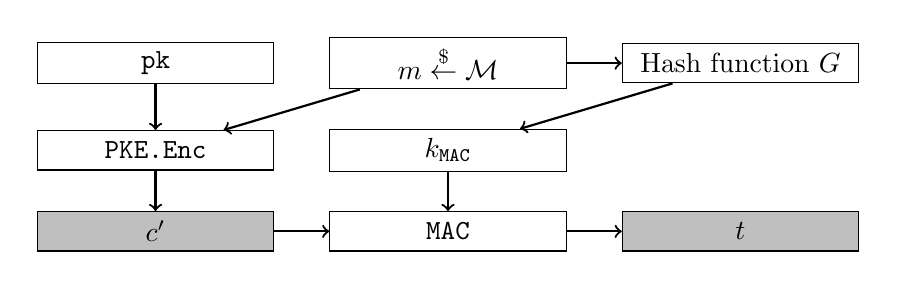
\begin{tikzpicture}
        \tikzstyle{rect} = [draw, rectangle, minimum width=3cm, minimum height=0.5cm]
        \tikzstyle{filledrect} = [draw, rectangle, minimum width=3cm, minimum height=0.5cm, fill=lightgray]
        \matrix [column sep=7mm, row sep=5mm] {
            \node (pk) [rect] {$\pk$}; &
            \node (m) [rect] {$m \leftsample \mathcal{M}$}; &
            \node (hashg) [rect] {Hash function $G$}; \\
            \node (pkeenc) [rect] {$\texttt{PKE.Enc}$}; &
            \node (mackey) [rect] {$k_\mac$}; \\
            \node (ct) [filledrect] {$c^\prime$}; &
            \node (mac) [rect] {$\mac$}; &
            \node (tag) [filledrect] {$t$}; \\
        };
        \draw[->, thick] (pk) -- (pkeenc);
        \draw[->, thick] (m) -- (pkeenc);
        \draw[->, thick] (m) -- (hashg);
        \draw[->, thick] (hashg) -- (mackey);
        \draw[->, thick] (pkeenc) -- (ct);
        \draw[->, thick] (mackey) -- (mac);
        \draw[->, thick] (ct) -- (mac);
        \draw[->, thick] (mac) -- (tag);
    \end{tikzpicture}

    \caption{Combining PKE with MAC using encrypt-then-MAC to ensure ciphertext integrity}\label{fig:etm-encap-data-flow}
\end{figure}

In Section \ref{sec:etm-construction} we will describe the encrypt-then-MAC KEM routines and state the security reduction. In Section \ref{sec:proof-of-etm-theorem} we present the proof reducing the IND-CCA security of the KEM tightly to the OW-PCA security of the underlying PKE and non-tightly to the unforgeability of the MAC. In Section \ref{sec:ow-pca-security} we discuss how the OW-PCA security of the PKE relates to the CCA security of the encrypt-then-MAC KEM. In Section \ref{sec:discussion-on-real-world-attacks} we discuss some generic attacks on our KEM transformation.

\subsection{The construction}\label{sec:etm-construction}
Let $\mathcal{B}^\ast$ denote the set of finite bit strings. Let $\mathcal{K}_\kem$ denote the set of all possible shared secrets. Let $(\keygen_\pke, \encrypt_\pke, \decrypt_\pke)$ be a PKE defined over message space $\mathcal{M}_\pke$ and ciphertext space $\mathcal{C}_\pke$. Let $\mac: \mathcal{K}_\mac \times \mathcal{B}^\ast \rightarrow \mathcal{T}$ be a MAC over key space $\mathcal{K}_\mac$ and tag space $\mathcal{T}$. Let $G: \mathcal{B}^\ast \rightarrow \mathcal{K}_\mac, H: \mathcal{B}^\ast \rightarrow \mathcal{K}_\kem$ be hash functions. The encrypt-then-MAC transformation $\etm[\pke,\mac,G,H]$ constructs a KEM $(\keygen_\etm, \encap_\etm, \decap_\etm)$ (Figure \ref{fig:etm-routines}).

\begin{figure}[h]
    \centering
    \begin{minipage}[t]{0.32\textwidth}
    \begin{algorithm}[H]
        \caption*{$\keygen_\etm()$}
        \begin{algorithmic}[1]
            \State $(\pk,  \sk) \leftsample \keygen_\pke()$
            \State $s \leftsample \mathcal{M}_\pke$
            \State $\sk \leftarrow (\sk, s)$
            \State \Return $(\pk, \sk)$
        \end{algorithmic}
    \end{algorithm}
    \end{minipage}\hfill
    \begin{minipage}[t]{0.3\textwidth}
    \begin{algorithm}[H]
        \caption*{$\encap_\etm(\pk)$}
        \begin{algorithmic}[1]
            \State $m \leftsample \mathcal{M}_\pke$
            \State $k \leftarrow G(m)$
            \State $c^\prime \leftsample \encrypt_\pke(\pk, m)$
            \State $t \leftarrow \mac(k, c^\prime)$
            \State $c \leftarrow (c^\prime, t)$
            \State $K \leftarrow H(m, c)$
            \State \Return $(c, K)$
        \end{algorithmic}
    \end{algorithm}
    \end{minipage}\hfill
    \begin{minipage}[t]{0.33\textwidth}
    \begin{algorithm}[H]
        \caption*{$\decap_\etm(\sk, c)$}
        \begin{algorithmic}[1]
            \Require $c = (c^\prime, t)$
            \Require $\sk = (\sk^\prime, s)$
            \State $\hat{m} \leftarrow \decrypt_\pke(\sk^\prime, c^\prime)$
            \State $\hat{k} \leftarrow G(\hat{m})$
            \If{$\mac(\hat{k}, c^\prime) = t$}
                \State $K \leftarrow H(\hat{m}, c)$
            \Else 
                \State $K \leftarrow H(s, c)$
            \EndIf
            \State \Return $K$
        \end{algorithmic}
    \end{algorithm}
    \end{minipage}
    \caption{The encrypt-then-MAC KEM routines}\label{fig:etm-routines}
\end{figure}

We chose to construct $\kem_\etm$ using implicit rejection $K \leftarrow H(s, c)$: on invalid ciphertexts, the decapsulation routine returns a fake shared secret that depends on the ciphertext and some secret values, though choosing to use explicit rejection should not impact the security of the KEM. In addition, because the underlying PKE can be randomized, the shared secret $K \leftarrow H(m, c)$ must depend on both the plaintext and the ciphertext. According to \cite{DBLP:conf/ima/Dent03,DBLP:conf/tcc/HofheinzHK17}, if the input PKE is \textit{rigid} (i.e. $m = \decrypt(\sk, c)$ if and only if $c = \encrypt(\pk, m)$), such as with RSA, then the shared secret may be derived from the plaintext alone $K \leftarrow H(m)$.

The CCA security of $\kem_\etm$ can be intuitively argued through an adversary's inability to learn additional information from the decapsulation oracle. For an adversary $A$ to produce a valid tag for some unauthenticated ciphertext $c^\prime$, it must either know the correct symmetric key or produce a forgery. Under the Random Oracle Model (ROM), $A$ cannot know the symmetric key without knowing its pre-image under the hash function $G$, so $A$ must either produced $c^\prime$ honestly, or have broken the one-wayness of the underlying PKE. This means that the decapsulation oracle will not leak information on decryption that the adversary does not already know. We formalize the security in Theorem \ref{thm:etm-is-ind-cca-secure}

\begin{theorem}\label{thm:etm-is-ind-cca-secure}
    For every IND-CCA adversary $A$ against $\kem_\etm$ that makes $q$ decapsulation queries, there exists a OW-PCA adversary $B$ against the underlying PKE making at least $q$ decapsulation queries, and an existential forgery adversary $C$ against the underlying MAC such that:

    \begin{equation*}
        \texttt{Adv}^\texttt{IND-CCA}_{\kem_\etm}(A) \leq q \cdot \texttt{Adv}_{\mac}(C) + 2 \cdot \texttt{Adv}^\texttt{OW-PCA}_{\pke}(B)
    \end{equation*}
\end{theorem}

\subsection{Proof of Theorem \ref{thm:etm-is-ind-cca-secure}}\label{sec:proof-of-etm-theorem}
We will prove Theorem \ref{thm:etm-is-ind-cca-secure} using a sequence of game. A summary of the the sequence of games can be found in Figure \ref{fig:etm-ind-cc2-sequence-of-games} and \ref{fig:ow-pca-simulates-game-3}. From a high level we made three incremental modifications to the IND-CCA game for $\kem_\etm$: \begin{enumerate}
    \item Replace the true decapsulation oracle with a simulated decapsulation oracle. The simulated decapsulation oracle does not directly decrypt the queried ciphertext. Instead it searches through the hash oracle and looks for matching queries using the plaintext-checking oracle. The true decapsulation oracle and the simulated decapsulation oracle disagree if and only if the adversary queries with a ciphertext that contains a forged MAC tag, so the adversary cannot distinguish the two games more than it can perform existential forgery against the underlying MAC.
    \item Replace the pseudorandom MAC key $k^\ast \leftarrow G(m^\ast)$ with a uniformly random MAC key $k^\ast \leftsample \mathcal{K}_\mac$. Under ROM, the adversary cannot distinguish this game from the previous one unless it queries the hash oracle with $m^\ast$, in which case a second adversary with access to a plaintext-checking oracle can win the OW-PCA game against the underlying PKE.
    \item Replace the pseudorandom shared secret $K_0 \leftarrow H(m^\ast, c)$ with a truly random shared secret $K_0 \leftsample \mathcal{K}_\kem$. Similar to the point above, the adversary cannot distinguish the change more than it can break the one-wayness of the underlying PKE. Furthermore, since both $K_0$ and $K_1$ are uniformly random, no adversary can have any advantage.
\end{enumerate}

A OW-PCA adversary can then simulate the modified IND-CCA game for the KEM adversary, and the advantage of the OW-PCA adversary is associated with the probability of certain behaviors of the KEM adversary.

\begin{figure}[h]
    \centering
    \begin{minipage}[t]{0.46\textwidth}
        \begin{algorithm}[H]
            \caption*{\texttt{IND-CCA} game for $\kem_\etm$}
            \begin{algorithmic}[1]
                \State $(\pk, \sk) \leftsample \keygen_\etm()$
                \State $m^\ast \leftsample \mathcal{M}$
                \State $c^\prime \leftsample \encrypt_\pke(\pk, m^\ast)$
                \State $k^\ast \leftarrow G(m^\ast)$
                    \Comment{Game 0-1}
                \State $k^\ast \leftsample \mathcal{K}_\mac$
                    \Comment{Game 2-3}
                \State $t \leftarrow \mac(k^\ast, c^\prime)$
                \State $c^\ast \leftarrow (c^\prime, t)$
                \State $K_0 \leftarrow H(m^\ast, c^\ast)$
                    \Comment{Game 0-2}
                \State $K_0 \leftsample \mathcal{K}_\kem$
                    \Comment{Game 3}
                \State $K_1 \leftsample \mathcal{K}_\kem$
                \State $b \leftsample \{0,1\}$
                \State $\hat{b} \leftarrow A^{\mathcal{O}^\decap}(\pk, c^\ast, K_b)$
                    \Comment{Game 0}
                \State $\hat{b} \leftarrow A^{\mathcal{O}^\decap_1}(\pk, c^\ast, K_b)$
                    \Comment{Game 1-3}
                \State \Return $\llbrack \hat{b} = b \rrbrack$
            \end{algorithmic}
        \end{algorithm}\vspace{-4em}
        \begin{algorithm}[H]
            \caption*{Hash oracle $\mathcal{O}^G(m)$}
            \begin{algorithmic}[1]
                \If{$\exists (\tilde{m}, \tilde{k}) \in \mathcal{L}^G : \tilde{m} = m$}
                    \State \Return $\tilde{k}$
                \EndIf
                \State $k \leftsample \mathcal{K}_\mac$
                \State $\mathcal{L}^G \leftarrow \mathcal{L}^G \cup \{(m, k)\}$
                \State \Return $k$
            \end{algorithmic}
        \end{algorithm}
    \end{minipage}
    \begin{minipage}[t]{0.53\textwidth}
        \begin{algorithm}[H]
            \caption*{Decap oracle $\mathcal{O}^\decap(c)$}
            \begin{algorithmic}[1]
                \State $(c^\prime, t) \leftarrow c$
                \State $\hat{m} = \decrypt_\pke(\sk^\prime, c^\prime)$
                \State $\hat{k} \leftarrow G(\hat{m})$
                \If{$\mac(\hat{k}, c^\prime) = t$}
                    \State $K \leftarrow H(\hat{m}, c)$
                \Else 
                    \State $K \leftarrow H(z, c)$
                \EndIf 
                \State \Return $K$
            \end{algorithmic}
        \end{algorithm}\vspace{-4em}
        \begin{algorithm}[H]
            \caption*{$\mathcal{O}^\decap_1(c)$}
            \begin{algorithmic}[1]
                \State $(c^\prime, t) \leftarrow c$
                \If{$
                    \exists (\tilde{m}, \tilde{k}) \in \mathcal{L}^G : 
                    \tilde{m} = \decrypt_\pke(\sk^\prime, c^\prime)
                    \land \mac(\tilde{k}, c^\prime) = t
                $}
                    \State $K \leftarrow H(\tilde{m}, c)$
                \Else
                    \State $K \leftarrow H(z, c)$
                \EndIf
                \State \Return $K$
            \end{algorithmic}
        \end{algorithm}\vspace{-4em}
        \begin{algorithm}[H]
            \caption*{$\mathcal{O}^H(m, c)$}
            \begin{algorithmic}[1]
                \If{$\exists (\tilde{m}, \tilde{c}, \tilde{K}) \in \mathcal{L}^H : \tilde{m} = m \land \tilde{c} = c$}
                    \State \Return $\tilde{K}$
                \EndIf
                \State $K \leftsample \mathcal{K}_\kem$
                \State $\mathcal{L}^H \leftarrow \mathcal{L}^H \cup \{(m, c, K)\}$
                \State \Return $K$
            \end{algorithmic}
        \end{algorithm}
    \end{minipage}
    \caption{Sequence of games in the proof of Theorem \ref{thm:etm-is-ind-cca-secure}}\label{fig:etm-ind-cc2-sequence-of-games}
\end{figure}
\begin{figure}[h]
    \begin{minipage}[t]{0.49\textwidth}
        \begin{algorithm}[H]
            \caption*{$B(\pk, {c^\prime}^\ast)$}
            \begin{algorithmic}[1]
                \State $z \leftsample \mathcal{M}$
                \State $k \leftsample \mathcal{K}_\mac$
                \State $t \leftarrow \mac(k, {c^\prime}^\ast)$
                \State $c^\ast \leftarrow ({c^\prime}^\ast, t)$
                \State $K \leftsample \mathcal{K}_\kem$
                \State $\hat{b} \leftarrow A^{
                    \mathcal{O}^\decap_B, \mathcal{O}^G_B, \mathcal{O}^H_B
                }(\pk, c^\ast, K)$
                \If{$\texttt{ABORT}(m)$}
                    \State \Return $m$
                \EndIf
            \end{algorithmic}
        \end{algorithm}\vspace{-4em}
        \begin{algorithm}[H]
            \caption*{$\mathcal{O}^H_B(m, c)$}
            \begin{algorithmic}
                \If{$\mathcal{O}^\pco(m, {c^\prime}^\ast) = 1$}
                    \State $\texttt{ABORT}(m)$
                \EndIf
                \If{$
                    \exists (\tilde{m}, \tilde{c}, \tilde{K}) \in \mathcal{L}^H 
                    : \tilde{m} = m \land \tilde{c} = c
                $}
                    \State \Return $\tilde{K}$
                \EndIf
                \State $K \leftsample \mathcal{K}_\kem$
                \State $\mathcal{L}^H \leftarrow \mathcal{L}^H \cup \{(m, c, K)\}$
                \State \Return $K$
            \end{algorithmic}
        \end{algorithm}
    \end{minipage}\hfill
    \begin{minipage}[t]{0.49\textwidth}
        \begin{algorithm}[H]
            \caption*{$\mathcal{O}^\decap_B(c)$}
            \begin{algorithmic}[1]
                \State $(c^\prime, t) \leftarrow c$
                \If{$\exists (\tilde{m}, \tilde{k}) \in \mathcal{L}^G : 
                    % \tilde{m} = \decrypt(\sk^\prime, c^\prime)
                    \mathcal{O}^\pco(\tilde{m}, c^\prime) = 1
                    \land \mac(\tilde{k}, c^\prime) = t
                $}
                    \State $K \leftarrow H(\tilde{m}, c)$
                \Else
                    \State $K \leftarrow H(z, c)$
                \EndIf
                \State \Return $K$
            \end{algorithmic}
        \end{algorithm}\vspace{-4em}
        \begin{algorithm}[H]
            \caption*{$\mathcal{O}^G_B(m)$}
            \begin{algorithmic}[1]
                \If{$\mathcal{O}^\pco(m, {c^\prime}^\ast) = 1$}
                    \State $\texttt{ABORT}(m)$
                \EndIf
                \If{$\exists (\tilde{m}, \tilde{k}) \in \mathcal{L}^G : \tilde{m} = m$}
                    \State \Return $\tilde{k}$
                \EndIf
                \State $k \leftsample \mathcal{K}_\mac$
                \State $\mathcal{L}^G \leftarrow \mathcal{L}^G \cup \{(m, k)\}$
                \State \Return $k$
            \end{algorithmic}
        \end{algorithm}
    \end{minipage}
    \caption{OW-PCA adversary $B$ simulates game 3 for IND-CCA adversary $A$ in the proof for Theorem \ref{thm:etm-is-ind-cca-secure}}\label{fig:ow-pca-simulates-game-3}
\end{figure}


\begin{proof}
    \emph{Game 0} is the standard KEM IND-CCA game. The decapsulation oracle $\mathcal{O}^\decap$ executes the decapsulation routine using the challenge keypair and return the results faithfully. The queries made to the hash oracles $\mathcal{O}^G, \mathcal{O}^H$ are recorded to their respective tapes $\mathcal{L}^G, \mathcal{L}^H$.

    \emph{Game 1} is identical to game 0 except that the true decapsulation oracle $\mathcal{O}^\decap$ is replaced with a simulated oracle $\mathcal{O}^\decap_1$. Instead of directly decrypting $c^\prime$ as in the decapsulation routine, the simulated oracle searches through the tape $\mathcal{L}^G$ to find a matching query $(\tilde{m}, \tilde{k})$ such that $\tilde{m}$ is the decryption of $c^\prime$. The simulated oracle then uses $\tilde{k}$ to validate the tag $t$ against $c^\prime$.

    If the simulated oracle accepts the queried ciphertext as valid, then there is a matching query that also validates the tag, which means that the queried ciphertext is honestly generated. Therefore, the true oracle must also accept the queried ciphertext. On the other hand, if the true oracle rejects the queried ciphertext, then the tag is simply invalid under the MAC key $k = G(\decrypt(\sk^\prime, c^\prime))$. Therefore, there could not have been a matching query that also validates the tag, and the simulated oracle must also rejects the queried ciphertext.

    This means that from the adversary $A$'s perspective, game 1 and game 0 differ only when the true oracle accepts while the simulated oracle rejects, which means that $t$ is a valid tag for $c^\prime$ under $k = G(\decrypt(\sk^\prime, c^\prime))$, but $k$ has never been queried. Under the random oracle model, such $k$ is a uniformly random sample of $\mathcal{K}_\mac$ that the adversary does not know, so for $A$ to produce a valid tag is to produce a forgery against the $\mac$ under an unknown and uniformly random key. Therefore, we can bound the probability that the true decapsulation oracle disagrees with the simulated oracle by the probability that some MAC adversary produces a forgery:

    \begin{equation*}
        P\left[\mathcal{O}^\decap(c) \neq \mathcal{O}^\decap_1(c)\right]
        \leq \adv_\texttt{MAC}(C).
    \end{equation*}

    Across all $q$ decapsulation queries, the probability that at least one query is a forgery is thus at most $q \cdot P\left[\mathcal{O}^\decap(c) \neq \mathcal{O}^\decap_1(c)\right]$. By the difference lemma:

    \begin{equation*}
        \left\vert \adv_{G_0}(A) - \adv_{G_1}(A) \right\vert\leq q\cdot  \adv_\texttt{MAC}(C).
    \end{equation*}

    \emph{Game 2} is identical to game 1, except that the challenger samples a uniformly random MAC key $k^\ast \leftsample \mathcal{K}_\mac$ instead of deriving it from $m^\ast$. From $A$'s perspective the two games are indistinguishable, unless $A$ queries $G$ with the value of $m^\ast$. Denote the probability that $A$ queries $G$ with $m^\ast$ by $P[\texttt{QUERY G}]$, then:

    \begin{equation*}
        \left\vert \adv_{G_1}(A) - \adv_{G_2}(A) \right\vert \leq P\left[\texttt{QUERY G}\right].
    \end{equation*}

    \emph{Game 3} is identical to game 2, except that the challenger samples a uniformly random shared secret $K_0 \leftsample \mathcal{K}_\kem$ instead of deriving it from $m^\ast$ and $t$. From $A$'s perspective the two games are indistinguishable, unless $A$ queries $H$ with $(m^\ast, \cdot)$. Denote the probability that $A$ queries $H$ with $(m^\ast, \cdot)$ by $P[\texttt{QUERY H}]$, then:

    \begin{equation*}
        \left\vert \adv_{G_2}(A) - \adv_{G_3}(A) \right\vert \leq P\left[\texttt{QUERY H}\right].
    \end{equation*}

    Since in game 3, both $K_0$ and $K_1$ are uniformly random and independent of all other variables, no adversary can have any advantage: $\adv_{G_3}(A) = 0$.

    We will bound $P[\texttt{QUERY G}]$ and $P[\texttt{QUERY H}]$ by constructing a OW-PCA adversary $B$ against the underlying PKE that uses $A$ as a sub-routine. $B$'s behaviors are summarized in Figure \ref{fig:ow-pca-simulates-game-3}.

    $B$ simulates game 3 for $A$: upon receiving the public key $\pk$ and challenge encryption ${c^\prime}^\ast$, $B$ samples random MAC key and session key to produce the challenge encapsulation, then feeds it to $A$. When simulating the decapsulation oracle, $B$ uses the plaintext-checking oracle to look for matching queries in $\mathcal{L}^G$. When simulating the hash oracles, $B$ uses the plaintext-checking oracle to detect when $m^\ast = \decrypt(\sk^\prime, {c^\prime}^\star)$ has been queried. When $m^\ast$ is queried, $B$ terminates $A$ and returns $m^\ast$ to win the OW-PCA game. In other words:

    \begin{equation*}
        \begin{aligned}
            P\left[\texttt{QUERY G}\right] &\leq \adv^\texttt{OW-PCA}_\pke(B), \\
            P\left[\texttt{QUERY H}\right] &\leq \adv^\texttt{OW-PCA}_\pke(B). \\
        \end{aligned}
    \end{equation*}

    Combining all equations above produce the desired security bound.
\end{proof}

\subsection{OW-PCA security}\label{sec:ow-pca-security}
In this section, we survey the OW-PCA security of various well-known PKE schemes and discuss the suitability of applying the encrypt-then-MAC KEM transformation. 

The security notion of \textit{one-wayness under plaintext-checking attack} (OW-PCA) was introduced by Okamoto and Pointcheval in \cite{DBLP:conf/ctrsa/OkamotoP01}, where the authors reduced the security of a generic CCA secure transformation (REACT) to the OW-PCA security of the input public-key cryptosystem. Following REACT, Pointcheval et al. proposed GEM \cite{DBLP:conf/ctrsa/CoronHJPPT02}, another generic CCA secure transformation whose security reduces to the OW-PCA security of the underlying PKE. Around the time REACT and GEM were published, the best known CCA secure transformation is Optimal Asymmetric Encryption Padding (OAEP)\cite{DBLP:conf/eurocrypt/BellareR94}. Compared to OAEP's requirement for one-way trapdoor permutation, OW-PCA security is easier to achieve: any one-way trapdoor permutation (such as RSA) is automatically OW-PCA secure, while there are cryptosystems that are OW-PCA secure but not one-way trapdoor permutation (Table \ref{tbl:ow-pca-candidates}). More recently, the modular Fujisaki-Okamoto transformation \cite{DBLP:conf/tcc/HofheinzHK17} proposed CCA secure KEM whose security reduces to the OW-PCA security of the input PKE under both ROM and QROM.

Theorem \ref{thm:etm-is-ind-cca-secure} stated that if the underlying PKE is OW-PCA secure, then the encrypt-then-MAC KEM is IND-CCA secure. Conversely, if the underlying PKE is not OW-PCA secure, then the encrypt-then-MAC KEM is not IND-CCA secure. This is captured in Lemma \ref{lemma:ind-cca-implies-ow-pca}

\begin{lemma}\label{lemma:ind-cca-implies-ow-pca}
    For every OW-PCA adversary $A$ against the underlying PKE, there exists an IND-CCA adversary $B$ against the encrypt-then-MAC KEM such that:
    \begin{equation*}
        \adv^\texttt{IND-CCA}_{\kem_\etm}(B) = \adv^\texttt{OW-PCA}_{\pke}(A)
    \end{equation*}
\end{lemma}

For a sketch of proof, we observe that the IND-CCA adversary $B$ can perfectly simulate the plaintext-checking oracle for the OW-PCA adversary $A$ (Figure \ref{fig:simulate-pca-oracle-with-cca-oracle}), and if $A$ succeeds in breaking the one-wayness of the underlying PKE, then $B$ can compute the shared secret associated with the challenge ciphertext, which allows $B$ to distinguish true shared secret from random bit strings.

\begin{figure}[h]
    \centering
    \begin{minipage}[t]{0.4\textwidth}
        \begin{algorithm}[H]
            \caption*{$\mathcal{O}^\pco_\decap(m, c^\prime)$}
            \begin{algorithmic}[1]
                \State $k \leftarrow G(m)$
                \State $t \leftarrow \mac(k, c^\prime)$
                \State $c \leftarrow (c^\prime, t)$
                \State $K \leftarrow H(m, c)$
                \State \Return $\llbrack \mathcal{O}^\decap(c) = K\rrbrack$
            \end{algorithmic}
        \end{algorithm}
    \end{minipage}
    \caption{Plaintext-checking oracle of the underlying PKE can be simulated using decapsulation oracle of the encrypt-then-MAC KEM. Let $c^\prime$ denote some PKE ciphertext. If $m$ is the decryption of $c^\prime$, then $m$ will hash into the correct MAC key and produce the correct tag $t$, and the decapsulation oracle will accept the KEM ciphertext $c = (c^\prime, t)$ and return the true shared secret $K = H(m, c)$. If $m$ is not the decryption of $c^\prime$, then the probability of producing the correct tag is negligible, and the decapsulation oracle will reject $(c^\prime, t)$.}\label{fig:simulate-pca-oracle-with-cca-oracle}
\end{figure}

For the remainder of this section, we will review the OW-PCA security of some well-known cryptosystems. A summary can be found in Table \ref{tbl:ow-pca-candidates}.

\begin{table}
    \centering
    \begin{tabular}{|p{9em}|p{10em}|p{14em}|}
        \hline
        \centering\textbf{PKE} & \textbf{Category} & \textbf{Is it OW-PCA?} \\
        \hline
        RSA & Number theoretic & Yes \cite{DBLP:conf/ima/Dent03,DBLP:journals/iacr/Shoup01} \\
        \hline
        ElGamal & {Number theoretic or \newline elliptic curve} & If Gap Diffie-Hellman assumption holds \cite{DBLP:conf/ctrsa/AbdallaBR01,DBLP:conf/pkc/OkamotoP01} \\
        \hline\hline
        FrodoKEM & Lattice-based & No, full key recovery \cite{DBLP:conf/crypto/GuoJN20,DBLP:conf/eurocrypt/BaetuDHTV19} \\
        \hline
        Kyber/Saber & Lattice-based & No, full key recovery \cite{DBLP:conf/acns/Huguenin-Dumittan20,DBLP:conf/asiacrypt/XagawaIUTH21,DBLP:conf/pqcrypto/GuoM23} \\
        \hline
        NTRU & Lattice-based & No, full key recovery \cite{hoffstein1999reaction,DBLP:conf/crypto/JaulmesJ00,DBLP:journals/tches/UenoXTITH22} \\
        \hline\hline
        HQC & Code-based & No, full key recovery \cite{DBLP:conf/acns/Huguenin-Dumittan20,DBLP:conf/eurocrypt/BaetuDHTV19} \\
        \hline
        BIKE & Code-based & No, partial key recovery \cite{DBLP:conf/asiacrypt/Guo0S16} \\
        \hline
        Classic McEliece & Code-based & Unknown, but there is no known attack \cite{DBLP:journals/tches/UenoXTITH22} \\
        \hline
    \end{tabular}
    \caption{The landscape of OW-PCA security}\label{tbl:ow-pca-candidates}
\end{table}



\subsubsection{Number-theoretic cryptosystems} The RSA cryptosystem as it was originally proposed in \cite{DBLP:journals/cacm/RivestSA78} is OW-PCA secure. This is because the RSA cryptosystem is a one-way trapdoor permutation \cite{DBLP:conf/crypto/FujisakiOPS01}, meaning that encryption and decryption are both injective. Given some public key $(N=pq, e)$ and a plaintext-ciphertext pair $(m, c)$, one can check that $m$ is the decryption of $c$ by checking that $c \equiv m^e \mod N$, which renders a plaintext-checking oracle completely useless.

The ElGamal cryptosystem \cite{DBLP:journals/tit/Elgamal85} is OW-PCA secure if the Gap Diffie-Hellman assumption \cite{DBLP:conf/pkc/OkamotoP01} holds for the underlying group (finite field or elliptic curve). This is the basis on which the CCA security of DHIES \cite{DBLP:conf/ctrsa/AbdallaBR01} is proved. We will discuss in detail in Section \ref{sec:application-to-elgamal}.

\subsubsection{Lattice-based cryptosystems} In many prominent cryptosystems based on the Learning with Error (LWE) problems, the plaintext is encrypted by adding noise. If an adversary adds additional noise to the ciphertext, the modified ciphertext may or may not decrypt back to the same plaintext. Querying the plaintext-checking oracle with modified ciphertexts containing varying amount of noise thus allows an adversary to recover the secret key. Such key-recovery plaintext-checking attacks (KR-PCA) were described for FrodoKEM in \cite{DBLP:conf/crypto/GuoJN20,DBLP:conf/eurocrypt/BaetuDHTV19}. Similar attacks for Kyber and Saber were described in \cite{DBLP:conf/acns/Huguenin-Dumittan20,DBLP:conf/asiacrypt/XagawaIUTH21,DBLP:conf/pqcrypto/GuoM23}. As Peikert pointed out in \cite{cryptoeprint:2014/070}, because of the search-decision equivalence of the (Ring) Learning With Error problem, lattice-based cryptosystems are unlikely to have inherent OW-PCA security. 

NTRU is another family of lattice-based cryptosystems. Hoffstein and Silverman \cite{hoffstein1999reaction} proposed KR-PCA for the original NTRU cryptosystem, which Ueno et al. \cite{DBLP:journals/tches/UenoXTITH22} adapted into a KR-PCA against modern instantiations such as NTRU-HPS and NTRU-HRSS (also see \cite{cryptoeprint:2021/168}). Ueno et al. also adapted \cite{DBLP:conf/crypto/JaulmesJ00} into a KR-PCA against NTRU-Prime.

\subsubsection{Code-based cryptosystems} HQC \cite{hamming-quasi-cyclic-4th-round-submission}, despite being based on hard coding problems, is structurally similar to lattice-based cryptosystems Kyber, Saber, etc. \cite{DBLP:journals/tches/UenoXTITH22}. Consequently, KR-PCA for lattice cryptosystems can be easily adapted to work on HQC \cite{DBLP:conf/acns/Huguenin-Dumittan20,DBLP:conf/eurocrypt/BaetuDHTV19}. BIKE \cite{bike-4th-round-submission} is based on the Niederreiter cryptosystem instantiated with quasi-cyclic moderate density parity check (QC-MDPC) code \cite{DBLP:conf/isit/MisoczkiTSB13}. \cite{DBLP:conf/asiacrypt/Guo0S16} described KR-PCA against QC-MDPC code, which can partially recover BIKE secret keys \cite{DBLP:conf/asiacrypt/XagawaIUTH21}. There is no known adaptive attack against Classic McEliece  \cite{DBLP:journals/tches/UenoXTITH22}.

\subsection{Additional implementation notes}\label{sec:discussion-on-real-world-attacks}
\subsubsection{Securely deriving MAC key} Because the MAC key is pseudorandomly derived from the PKE plaintext (instead of uniformly and independently sampled), it is possible to construct a large lookup table mapping each PKE plaintext to a MAC key, then check the KEM ciphertext $(c, t)$ against each MAC key to recover the pre-image. As was pointed out in \cite{DBLP:journals/iacr/Bernstein21,cryptoeprint:2021/912}, this relationship between the MAC tag and the PKE plaintext could damage the security of the scheme. This can be mitigated by including the PKE public key when deriving the MAC key $k_\mac \leftarrow G(\pk, m)$ or even including random salt at each encapsulation $k_\mac \leftarrow G(\pk, m, \text{salt})$, which can increase the cost of such dictionary attacks.

\subsubsection{One-time MAC} When the encrypt-then-MAC KEM is instantiated with a PKE with a sufficiently large plaintext space, we expect the probability of two encapsulations sampling the same PKE plaintext to be negligible within some reasonable keypair lifetime, and if the hash function is collision resistant, then the probability of two encapsulations deriving the same MAC key is also negligible. Therefore, we speculate that the encrypt-then-MAC KEM can be instantiated with one-time MACs \cite{DBLP:journals/jcss/CarterW79} with no security impact, while one-time MACs can be computationally more efficient than many-time secure MACs (e.g., DHIES proposed to use HMAC and CBC-MAC \cite{DBLP:conf/ctrsa/AbdallaBR01}).

\subsubsection{Deriving shared secret} If the decryption routine of the underlying PKE is not injective, then the shared secret must be derived from both the PKE plaintext and the ciphertext: if the shared secret is derived from the plaintext alone, and the KEM adversary $A$ can find a modified ciphertext that decrypts back to the same PKE plaintext, then $A$ can query the decapsulation oracle with the modified ciphertext and obtain the true decapsulation. However, the shared secret does not have to be derived from hashing the entire ciphertext. Instead, we propose to derive the shared secret from the MAC tag, which is functionally equivalent to a keyed hash of the ciphertext. Since the MAC tag is usually much smaller than the ciphertext, hashing the tag instead of the entire ciphertext can lead to a noticeable  speedup.

\section{Applying encrypt-then-MAC to code-based cryptosystem}\label{sec:application-to-mceliece}
{\it Background.} Code-based cryptography was introduced by Robert J. McEliece in 1978 \cite{McEliece1978}. The McEliece cryptosystem samples a random $(n, k)$-linear code over some finite field $\mathbb{F}$ with generator matrix $G \in \mathbb{F}^{n \times k}$, then generates the public key by scrambling the generator matrix $\pk = G^\prime \leftarrow P \cdot G \cdot S$ using a secret permutation matrix $P \in \mathbb{F}^{n \times n}$ and a secret invertible matrix $S\in\mathbb{F}^{k \times k}$. Because $P$ and $S$ are both invertible, $G^\prime$ is also a generator matrix for an $(n, k)$-linear code. The secret key consists of the decoding routine, the secret permutation matrix, and the secret invertible matrix. A plaintext message $m$ is encrypted by first encoding it using $G^\prime$, then adding an error vector $\mathbf{e}$ to the codeword: $c \leftarrow G^\prime\cdot m + \mathbf{e}$. To decrypt a ciphertext, the permutation is first removed, then the error vector is removed using the decoding routine, and finally, the message is recovered. The one-wayness of the McEliece cryptosystem reduces to the NP-hard problem of decoding a random linear code \cite{DBLP:journals/tit/BerlekampMT78}. Harald Niederreiter improved the efficiency of the McEliece cryptosystem in 1986 \cite{niederreiter1986knapsack} by replacing the generator matrix of a random linear code with the parity-check matrix. Correspondingly, the plaintext space becomes the set of fixed-weight error vectors, which are encrypted by computing the syndrome under the parity-check matrix, $c \leftarrow H\mathbf{e}$. The one-wayness of the Niederreiter variant reduces to the syndrome decoding problem, which is proven NP-hard \cite{DBLP:journals/tit/BerlekampMT78}. Compared to the McEliece formulation, the Niederreiter variant enjoys a smaller public key and smaller ciphertexts.

\textit{Remark.} There are three code-based post-quantum KEM candidates in the fourth round of NIST's PQC standardization project: HQC \cite{hamming-quasi-cyclic-4th-round-submission}, BIKE \cite{bike-4th-round-submission}, and Classic McEliece \cite{ClassicMcEliece2022}. As discussed in Section \ref{sec:ow-pca-security}, there exist full or partial key recovery plaintext checking attacks against HQC and BIKE. While there is no rigorous proof that Classic McEliece is OW-PCA, there is also no known plaintext checking attack. The CCA security of instantiating the encrypt-then-MAC KEM with Classic McEliece is thus based on the conjectured OW-PCA security of the one-way subroutines described in Section \ref{sec:classic-mceliece}.

\subsection{Construction of McElieceEtM}\label{sec:classic-mceliece}
%\subsection{Classic McEliece}\label{sec:classic-mceliece}
Classic McEliece \cite{ClassicMcEliece2022} is an IND-CCA secure post-quantum KEM submitted to the PQC standardization project and is currently one of three viable fourth-round KEM candidates. Classic McEliece is constructed in two layers. The first layer is a OW-CPA secure PKE based on the Niederreiter cryptosystem using a random binary Goppa code, and the second layer is a modified Fujisaki-Okamoto transformation. Each instance of Classic McEliece is parameterized by the base field size $m$ (which induces a finite field with order $q = 2^m$), the codeword size $n$, and the error vector weight $t$.

\begin{figure}[hp]
\begin{algorithm}[H]
    \caption{$\texttt{SeededKeyGen}(\delta)$}\label{alg:mceliece-seeded-keygen}
    \begin{algorithmic}[1]
        \Require $l$-bit seed $\delta$
        \State Expand $\delta$ to $n + \sigma_2 q + \sigma_1 t + l$ bits, where $\delta_1 = 16, \delta_2 = 32$
        \State Denote the last $l$ bits by $\delta^\prime$
        \State Denote the first $n$ bits by $s$
        \State Compute $\alpha_0, \ldots, \alpha_{q-1}$ from the next $\sigma_2 q$ bits using the \texttt{FieldOrdering} algorithm. If this fails, set $\delta \leftarrow \delta^\prime$ and restart
        \State Compute $g$ from the next $\delta_1 t$ bits using the \texttt{Irreducible} algorithm. If this fails, set $\delta \leftarrow \delta^\prime$ and restart
        \State $\Gamma \leftarrow (g, \alpha_0, \alpha_1, \ldots, \alpha_{n-1})$
        \State Compute $(T, c_{mt-\mu}, \ldots, c_{mt-1}, \Gamma^\prime) \leftarrow \texttt{MatGen}(\Gamma)$. If this fails, set $\delta \leftarrow \delta^\prime$ and restart
        \State Write $\Gamma^\prime$ as $(g, \alpha_0^\prime, \alpha_1^\prime, \ldots, \alpha_{n-1}^\prime)$
        \State Set $\alpha = (\alpha_0^\prime, \ldots, \alpha_{n-1}^\prime, \alpha_n, \ldots, \alpha_{q-1})$ and $c = (c_{mt-\mu}, \ldots, c_{mt-1})$
        \State Output $T$ as the public key and $(\delta, c, g, \alpha, s)$ as private key
    \end{algorithmic}
\end{algorithm}
\vspace{-4em}
\begin{algorithm}[H]
    \caption{$\texttt{Encode}(T, \mathbf{e})$}\label{alg:mceliece-encode}
    \begin{algorithmic}[1]
        \Require Public key $T\in\mathbb{F}_2^{mt \times (n - mt)}$
        \Require Weight-t vector $\mathbf{e}\in\mathbb{F}_2^n$
        \State Define $H = (I_{mt} \mid T)$
        \State Compute and return $\mathbf{c} \leftarrow H\mathbf{e} \in \mathbb{F}_2^{mt}$
    \end{algorithmic}
\end{algorithm}
\vspace{-4em}
\begin{algorithm}[H]
    \caption{$\texttt{Decode}(\Gamma, \mathbf{c})$}\label{alg:mceliece-decode}
    \begin{algorithmic}[1]
        \Require Secret key $\Gamma = (g, \alpha_0, \ldots, \alpha_{n-1})$
        \Require Syndrome $\mathbf{c}\in\mathbb{F}_2^{mt}$
        \State Extend $\mathbf{c}$ to $\mathbf{v} \in\mathbb{F}_2^n$ by appending 0's 
        \State Find the unique Goppa codeword $\mathbf{w}\in\mathbb{F}_2^n$ such that $H\mathbf{w} = 0$ and $\mathbf{w}$ has Hamming distance no more than $t$ from $\mathbf{v}$. If there is no such $\mathbf{w}$, return $\bot$
        \State \Return  $\mathbf{e} \leftarrow \mathbf{v} + \mathbf{w}$
    \end{algorithmic}
\end{algorithm}
\vspace{-4em}
\begin{algorithm}[H]
    \caption{$\texttt{Encap}(\pk)$}\label{alg:mceliece-encap}
    \begin{algorithmic}[1]
        \Require Public key $\pk = T\in\mathbb{F}_2^{mt \times (n - mt)}$
        \State Use \texttt{FixedWeight} to generate a vector $\mathbf{e} \in \mathbf{F}_2^n$ with Hamming weight $t$
        \State Compute $\mathbf{c} \leftarrow \texttt{Encode}(T, \mathbf{e})$
        \State Compute $K \leftarrow H(1, \mathbf{e}, \mathbf{c})$
        \State \Return $(\mathbf{c}, K)$
    \end{algorithmic}
\end{algorithm}
\vspace{-4em}
\begin{algorithm}[H]
    \caption{$\texttt{Decap}(\sk, \mathbf{c})$}\label{alg:mceliece-decap}
    \begin{algorithmic}[1]
        \Require Secret key $\sk$ contains $s \in \mathbb{F}_2^n$ and $\Gamma = (g, \alpha_0, \alpha_1, \ldots, \alpha_{n-1})$
        \Require Ciphertext $\mathbf{c} \in \mathbb{F}_2^{mt}$
        \State Set $b \leftarrow 1$
        \State Compute $\mathbf{e} \leftarrow \texttt{Decode}(\Gamma, \mathbf{c})$
        \If{$\wt(\mathbf{e})\neq t \lor H\mathbf{e}\neq\mathbf{c}$}
            \State Set $\mathbf{e} \leftarrow s, b \leftarrow 0$
        \EndIf
        \State \Return $K \leftarrow H(b, \mathbf{e}, \mathbf{c})$
    \end{algorithmic}
\end{algorithm}
\end{figure}

Algorithm \ref{alg:mceliece-seeded-keygen} describes the key generation routine of Classic McEliece. In step 4, \texttt{FieldOrdering} takes the input bits and outputs either $\bot$ or a sequence $(\alpha_0, \ldots, \alpha_{q-1})$ distinct elements of $\mathbb{F}_q$. In step 5, \texttt{Irreducible}  takes the input bits and outputs either $\bot$ or a monic irreducible degree-$t$ polynomial $g \in \mathbb{F}_q[x]$. In step 7, \texttt{MatGen} outputs either $\bot$ or an $mt \times k$ matrix over $\mathbb{F}_2$. We refer readers to \cite{ClassicMcEliece2022} for details of these subroutines.

Algorithms \ref{alg:mceliece-encode} and \ref{alg:mceliece-decode} describe the encoding and decoding subroutines of the Niederreiter layer. Note that our description of the decoding routine differs from \cite{ClassicMcEliece2022} in that we did not include the weight and/or re-encryption check. Instead, they are included in the description of the decapsulation subroutines (Algorithm \ref{alg:mceliece-decap}). This is because we later plan to substitute these checks with computing a MAC tag when applying the encrypt-then-MAC KEM transformation.

Algorithms \ref{alg:mceliece-encap} and \ref{alg:mceliece-decap} describe Classic McEliece's KEM construction using the CPA secure Niedereitter cryptosystem described above. In step 1 of Algorithm \ref{alg:mceliece-encap}, \texttt{FixedWeight} samples a random vector $\mathbf{e}\in\mathbb{F}_2^n$ with Hamming weight $t$. In this KEM construction, Classic McEliece makes use of re-encryption (step 3 of Algorithm \ref{alg:mceliece-decap}) to ensure the integrity of the ciphertext. \vspace{0.1cm}

\noindent{\bf Subroutines of McElieceEtM.} We instantiate the encrypt-then-MAC KEM transformation using \texttt{SeededKeyGen}, \texttt{FixedWeight}, \texttt{Encode}, and \texttt{Decode} as subroutines. The result is called McElieceEtM. Figure \ref{fig:mceliece-plus} presents the encapsulation and decapsulation routines of McElieceEtM. Its key generation routine is identical to the key generation of Classic McEliece. Its encapsulation derives a MAC key from the output of \texttt{FixedWeight} and signs the syndrome computed from \texttt{Encode}. In decapsulation, weight and syndrome check is replaced with re-deriving the MAC key and checking the tag.

\begin{figure}[h]
    \centering
    
    \begin{minipage}[t]{0.48\textwidth}
        \begin{algorithm}[H]
            \caption{$\encap_\text{McElieceEtM}(\pk)$}
            \begin{algorithmic}[1]
                \Require Public key $\pk = T \in\mathbb{F}_2^{mt \times n}$
                \State $\mathbf{e} \leftsample \texttt{FixedWeight}()$
                \State $k \leftarrow G(\mathbf{e})$
                \State $\mathbf{c} \leftarrow \texttt{Encode}(T, \mathbf{e})$
                \State $t \leftarrow \mac(k, c)$
                \State $K \leftarrow H(\mathbf{e}, \mathbf{c})$
                \State \Return $(\mathbf{c}, K)$
            \end{algorithmic}
        \end{algorithm}
    \end{minipage}\hfill
    \begin{minipage}[t]{0.48\textwidth}
        \begin{algorithm}[H]
            \caption{$\decap_\text{McElieceEtM}(\sk, c)$}
            \begin{algorithmic}[1]
                \Require Secret key $\sk = (\Gamma, s)$
                \Require Ciphertext $c = (\mathbf{c}, t)$
                \State $\hat{\mathbf{e}} \leftarrow \texttt{Decode}(\Gamma, \mathbf{c})$
                \State $\hat{k} \leftarrow G(\hat{\mathbf{e}})$
                \If{$\mac(\hat{k}, \mathbf{c}) \neq t$}
                    \State $K \leftarrow H(s, \mathbf{c})$
                \Else
                    \State $K \leftarrow H(\mathbf{e}, \mathbf{c})$
                \EndIf
                \State\Return $K$
            \end{algorithmic}
        \end{algorithm}
    \end{minipage}

    \caption{McElieceEtM: applying encrypt-then-MAC to the Niedereitter cryptosystem}\label{fig:mceliece-plus}
\end{figure}

\subsection{Choosing MAC}\label{sec:choosing-mac}
For a concrete instantiation of McElieceEtM, we chose four MACs covering a variety of architectures. All MACs are parameterized with a 256-bit key and 128-bit tag, except for KMAC256, which can have a variable key and tag length.

\paragraph{Poly1305 \cite{DBLP:conf/fse/Bernstein05} and GMAC \cite{NIST80038D}} are both Carter-Wegman style MACs \cite{DBLP:journals/jcss/CarterW79,DBLP:journals/jcss/WegmanC81}, which compute the tag using finite field arithmetic. It first parses the message into a sequence of finite field elements, then evalutes a polynomial whose coefficients are the message blocks and whose indeterminate is the secret key. Specifically, Poly1305 oerates in the prime field $\mathbb{F}_q$ where $q = 2^{130} - 5$. GMAC operates in the binary extension field $\mathbb{F}_{2^{128}}$.

In our implementation, we used {\tt OpenSSL 3.3.1}'s \texttt{EVP\_MAC} interface. Within this interface, the Poly1305 implementation does not include a nonce and is thus only one-time secure. On the other hand, GMAC is implemented by passing all data into the associated data field of the authenticated encryption scheme AES-256-GCM. Assuming that nonce does not repeat within the lifetime of the symmetric key, GMAC is many-time secure.

\paragraph{CMAC \cite{NIST80038B}} is based on the CBC-MAC \cite{DBLP:conf/crypto/BlackR00}. To compute a CMAC tag, the message is first padded and parsed into blocks. Each block is first XOR'ed with the previous block's output, then encrypted under a block cipher using the secret key. The final output is XOR'ed with a sub-key derived from the secret key before being encrypted for one last time. In our implementation, the block cipher is instantiated with AES-256, which makes it particularly suitable for embedded devices with constrainted computing capacity but hardware support for AES. CMAC is many-time secure.

\paragraph{KMAC256 \cite{NIST800185}} is a pseudorandom function and keyed hash function based on \textit{KECCAK} \cite{NISTFIPS202}, although unlike SHAKE, altering the requested output length generates a new unrelated output. KMAC256 is slower than other MACs, but it is the only construction with a flexible key and tag length. We fixed the key length at 256 bits, and varied the tag length to 128, 192, and 256 bits depending on the desired security levels.

\paragraph{Remark} There are new lightweight MACs such as EliMAC \cite{DBLP:journals/tosc/DobraunigMN23}, LightMAC \cite{DBLP:conf/fse/LuykxPTY16}, and ZMAC \cite{DBLP:conf/crypto/IwataMPS17}, which may offer a better performance than the MACs listed above. However, the performance of the encrypt-then-MAC KEM is dominated by the public-key cryptographic operations and the key-derivation functions. For KEMs with a relatively short ciphertext, such as Classic McEliece, the performance impact of the MAC is insignificant.

\subsection{Performance benchmark}
The subroutines \texttt{SeededKeyGen}, \texttt{FixedWeight}, \texttt{Encode}, and \texttt{Decode} were taken from the \texttt{vec} implementation submitted to the fourth round of NIST PQC standardization project\footnote{\url{https://csrc.nist.gov/csrc/media/Projects/post-quantum-cryptography/documents/round-4/submissions/mceliece-Round4.tar.gz}}. While there are a total of 10 sets of parameters in Classic McEliece (see Section \ref{sec:classic-mceliece-parameter-sets}), we only modified the 5 standard parameter variants. The only difference between the standard variants and the f-variants is the key generation routine, which is not the focus of this paper. Key pairs are fully interoperable between the standard and the f-variants, and the encapsulation/decapsulation routines are entirely identical.

We implement the McElieceEtM KEM in the {\tt C} language to benchmark the encapsulation and decapsulation algorithms for above four different MACs.  
We leverate the MAC implementations from {\tt OpenSSL 3.5.0}. Our C code is compiled using Apple Clang 15.0.0. The performance measurement is run on Apple Silicon M1 chip. The CPU clock is measured using \texttt{mach\_absolute\_time}. Each routine is run 10000 times, with median times reported in Table \ref{tbl:mceliece-plus-performance}.

\begin{table}[hp]
    \centering
    % \footnotesize
    \begin{tabular}[c]{|c|c|c|c|}
        \hline
        KEM & \texttt{Enc} & \texttt{Dec} & \texttt{Enc + Dec} \\
        \hline
        \texttt{mceliece348864} & 215 & 2471 & 2686 \\
        \hline
        \texttt{mceliece348864 + poly1305} & 316 (+46.98\%) & 2074 (-16.07\%) & 2390 (-11.02\%) \\
        \hline
        \texttt{mceliece348864 + gmac} & 335 (+55.81\%) & 2087 (-15.54\%) & 2422 (-9.83\%) \\
        \hline
        \texttt{mceliece348864 + cmac} & 340 (+58.14\%) & 2092 (-15.34\%) & 2432 (-9.46\%) \\
        \hline
        \texttt{mceliece348864 + kmac256} & 304 (+41.40\%) & 2093 (-15.30\%) & 2397 (-10.76\%) \\
        \hline
    \end{tabular}\vspace{1em}
    \begin{tabular}[c]{|c|c|c|c|}
        \hline
        KEM & \texttt{Enc} & \texttt{Dec} & \texttt{Enc + Dec} \\
        \hline
        \texttt{mceliece460896} & 487 & 6694 & 7181 \\
        \hline
        \texttt{mceliece460896 + poly1305} & 514 (+5.54\%) & 5784 (-13.59\%) & 6298 (-12.30\%) \\
        \hline
        \texttt{mceliece460896 + gmac} & 565 (+16.02\%) & 5809 (-13.22\%) & 6374 (-11.24\%) \\
        \hline
        \texttt{mceliece460896 + cmac} & 544 (+11.70\%) & 5905 (-11.79\%) & 6449 (-10.19\%) \\
        \hline
        \texttt{mceliece460896 + kmac256} & 570 (+17.04\%) & 5760 (-13.95\%) & 6330 (-11.85\%) \\
        \hline
    \end{tabular}\vspace{1em}
    \begin{tabular}[c]{|c|c|c|c|}
        \hline
        KEM & \texttt{Enc} & \texttt{Dec} & \texttt{Enc + Dec} \\
        \hline
        \texttt{mceliece6688128} & 816 & 7500 & 8316 \\
        \hline
        \texttt{mceliece6688128 + poly1305} & 889 (+8.95\%) & 6509 (-13.21\%) & 7398 (-11.04\%) \\
        \hline
        \texttt{mceliece6688128 + gmac} & 890 (+9.07\%) & 6521 (-13.05\%) & 7411 (-10.88\%) \\
        \hline
        \texttt{mceliece6688128 + cmac} & 900 (+10.29\%) & 6540 (-12.80\%) & 7440 (-10.53\%) \\
        \hline
        \texttt{mceliece6688128 + kmac256} & 901 (+10.42\%) & 6546 (-12.72\%) & 7447 (-10.45\%) \\
        \hline
    \end{tabular}\vspace{1em}
    \begin{tabular}[c]{|c|c|c|c|}
        \hline
        KEM & \texttt{Enc} & \texttt{Dec} & \texttt{Enc + Dec} \\
        \hline
        \texttt{mceliece6960119} & 699 & 7262 & 7961 \\
        \hline
        \texttt{mceliece6960119 + poly1305} & 735 (+5.15\%) & 6389 (-12.02\%) & 7124 (-10.51\%) \\
        \hline
        \texttt{mceliece6960119 + gmac} & 753 (+7.73\%) & 6450 (-11.18\%) & 7203 (-9.52\%) \\
        \hline
        \texttt{mceliece6960119 + cmac} & 763 (+9.16\%) & 6428 (-11.48\%) & 7191 (-9.67\%) \\
        \hline
        \texttt{mceliece6960119 + kmac256} & 765 (+9.44\%) & 6303 (-13.21\%) & 7068 (-11.22\%) \\
        \hline
    \end{tabular}\vspace{1em}
    \begin{tabular}[c]{|c|c|c|c|}
        \hline
        KEM & \texttt{Enc} & \texttt{Dec} & \texttt{Enc + Dec} \\
        \hline
        \texttt{mceliece8192128} & 858 & 7464 & 8322 \\
        \hline
        \texttt{mceliece8192128 + poly1305} & 955 (+11.31\%) & 6547 (-12.29\%) & 7502 (-9.85\%) \\
        \hline
        \texttt{mceliece8192128 + gmac} & 957 (+11.54\%) & 6550 (-12.25\%) & 7507 (-9.79\%) \\
        \hline
        \texttt{mceliece8192128 + cmac} & 945 (+10.14\%) & 6546 (-12.30\%) & 7491 (-9.99\%) \\
        \hline
        \texttt{mceliece8192128 + kmac256} & 957 (+11.54\%) & 6574 (-11.92\%) & 7531 (-9.50\%) \\
        \hline
    \end{tabular}\vspace{1em}
    \caption{McElieceEtM achieves 9-12\% speedup in combined ``encapsulate + decapsulate'' compared to Classic McEliece}\label{tbl:mceliece-plus-performance}
\end{table}

\section{Application to ElGamal}\label{sec:application-to-elgamal}
Applying the encrypt-then-MAC KEM transformation to the ElGamal cryptosystem results in a construction that is highly similar to DHIES \cite{DBLP:conf/ctrsa/AbdallaBR01}. In this section, we will show that the encrypt-then-MAC KEM transformation is a generalization of DHIES by showing that the Gap Diffie-Hellman assumption is a special case of OW-PCA security. Specifically, we sketch a proof of the following lemma.

\begin{lemma}\label{lemma:elgamal-is-ow-pca}
    For every OW-PCA adversary $A$ against the ElGamal cryptosystem, there exists a Gap Diffie-Hellman problem solver $B$ such that:

    \begin{equation*}
        \text{Adv}_\text{GapDH}(B) = \text{Adv}_\text{ElGamal}^\texttt{OW-PCA}(A).
    \end{equation*}
\end{lemma}

Each ElGamal cryptosystem \cite{DBLP:journals/tit/Elgamal85} is parameterized by a cyclic group $G = \langle g \rangle$ of prime order $q > 2$. A summary of the routine is shown in Figure \ref{fig:elgamal-routines}:

\begin{figure}[H]
    \centering

    \begin{minipage}[t]{0.32\textwidth}
        \begin{algorithm}[H]
            \caption*{\texttt{KeyGen()}}
            \begin{algorithmic}[1]
                \State $x \leftsample \mathbb{Z}_q$
                \State $\sk \leftarrow x$
                \State $\pk \leftarrow g^x$
                \State \Return $(\pk, \sk)$
            \end{algorithmic}
        \end{algorithm}
    \end{minipage}\hfill
    \begin{minipage}[t]{0.31\textwidth}
        \begin{algorithm}[H]
            \caption*{$\encrypt(\pk, m)$}
            \begin{algorithmic}[1]
                \Require $m \in G$
                \Require $\pk = g^x \in G$
                \State $y \leftsample \mathbb{Z}_q$
                \State $w \leftarrow g^y$
                \State $v \leftarrow m \cdot (g^x)^y$
                \State \Return $(w, v)$
            \end{algorithmic}
        \end{algorithm}
    \end{minipage}\hfill
    \begin{minipage}[t]{0.35\textwidth}
        \begin{algorithm}[H]
            \caption*{$\decrypt(\sk, c)$}
            \begin{algorithmic}[1]
                \Require $\sk = x \in \mathbb{Z}_q$
                \Require $c = (w, v) \in G \times G$
                \State $\hat{m} \leftarrow (w^x)^{-1}\cdot v$
                \State \Return $\hat{m}$
            \end{algorithmic}
        \end{algorithm}
    \end{minipage}
    
    \caption{ElGamal cryptosystem over cyclic group $G = \langle g \rangle$ of prime order $q$}\label{fig:elgamal-routines}
\end{figure}

The security of ElGamal cryptosystem reduces to the conjectured intractability of the computational and decisional Diffie-Hellman problem:

\begin{definition}[\textbf{computational Diffie-Hellman problem}]
    Let $x, y \leftsample \mathbb{Z}_q$ be uniformly random samples. Given $(g, g^x, g^y)$, compute $g^{xy}$.
\end{definition}
\begin{definition}[\textbf{decisional Diffie-Hellman problem}]
    Let $x, y, z \leftsample \mathbb{Z}_q$ be uniformly random samples. Let $h \leftsample \{g^z, g^{xy}\}$ be randomly chosen between $g^z$ and $g^{xy}$. Given $(g, g^x, g^y, h)$, determine whether $h$ is $g^{xy}$ or $g^z$. 
\end{definition}

It is also conjectured in \cite{DBLP:conf/ctrsa/AbdallaBR01} (and later extensively studied in \cite{DBLP:conf/pkc/OkamotoP01}) that for the certain choice of cyclic group $G$, the computational Diffie-Hellman problem remains intractable even if the adversary as access to a restricted decisional Diffie-Hellman oracle. This assumption is captured in the Gap Diffie-Hellman problem:

\begin{definition}[\textbf{Gap Diffie-Hellman problem}]
    Let $G = \langle g \rangle$ be a cyclic group of prime order $q > 2$. Let $x, y \leftsample \mathbb{Z}_q$ be uniformly random samples. Given $(g, g^x, g^y)$ and a restricted DDH oracle $\mathcal{O}^\text{DDH}: (u, v) \mapsto \llbrack u^x = v \rrbrack$, compute $g^{xy}$.
\end{definition}

We now present the proof for Lemma \ref{lemma:elgamal-is-ow-pca}. 
\begin{proof}
    We will prove by a sequence of games. A summary can be found in Figure \ref{fig:elgamal-pca-games}

    \begin{figure}[h]
        \centering

        \begin{minipage}[t]{0.4\textwidth}
            \begin{algorithm}[H]
                \caption*{$G_0 - G_2$}
                \begin{algorithmic}[1]
                    \State $x \leftsample \mathbb{Z}_q$
                    \State $m^\ast \leftsample G$
                    \State $y \leftsample \mathbb{Z}_q, w \leftarrow g^y$
                    \State $v \leftarrow m^\ast \cdot (g^x)^y$
                        \Comment{$G_0$ - $G_1$}
                    \State $v \leftsample G$
                        \Comment{$G_2$}
                    \State $c^\ast \leftarrow (w, v)$
                    \State $\hat{m} \leftsample A^{\pco}(g^x, c^\ast)$
                        \Comment{$G_0$}
                    \State $\hat{m} \leftsample A^{\pco_1}(g^x, c^\ast)$
                        \Comment{$G_1$ - $G_2$}
                    \State \Return $\llbrack \hat{m} = m^\ast \rrbrack$
                        \Comment{$G_0$ - $G_1$}
                    \State \Return $\llbrack \hat{m} = w^{-x}\cdot v \rrbrack$
                        \Comment{$G_2$}
                \end{algorithmic}
            \end{algorithm}
        \end{minipage}
        \begin{minipage}[t]{0.4\textwidth}
            \begin{algorithm}[H]
                \caption*{$\mathcal{O}^\pco(m, c=(w, v))$}
                \begin{algorithmic}[1]
                    \State \Return $\llbrack m = (w^x)^{-1}\cdot v\rrbrack$
                \end{algorithmic}
            \end{algorithm}
            \begin{algorithm}[H]
                \caption*{$\mathcal{O}^\pco_1(m, c=(w, v))$}
                \begin{algorithmic}[1]
                    \State \Return $\llbrack (w^x) = m^{-1} \cdot v \rrbrack$
                \end{algorithmic}
            \end{algorithm}
        \end{minipage}

        \caption{ The sequence of games in proving Lemma \ref{lemma:elgamal-is-ow-pca}}\label{fig:elgamal-pca-games}
    \end{figure}

    \emph{Game 0} is the OW-PCA game. Adversary $A$ has access to the plaintext-checking oracle $\mathcal{O}^\pco$ and wins the game if it can correctly recover the challenge plaintext $m^\ast$.

    \emph{Game 1} is identical to game 0, except that the formulation of the $\mathcal{O}^\pco$ is changed. When servicing the plaintext-checking query $(m, c = (w, v))$, $\pco_1$ checks whether $w^x$ is equal to $m^{-1} \cdot v$. Observe that in the cyclic group $G$, the algebraic expressions in $\mathcal{O}^\pco$ and $\mathcal{O}^\pco_1$ are equivalent, which means that $\mathcal{O}^\pco_1$ behaves identically to $\mathcal{O}^\pco$.

    \emph{Game 2} is identical to game 1 except for two modifications: first, when computing the challenge ciphertext, $v$ is no longer computed from $m^\ast$ but is randomly sampled; second, the win condition changed from $\hat{m} = m^\ast$ to $\hat{m} = w^{-x}\cdot v$. It is easy to verify that Game 0 through Game 2 are algebraically equivalent:

    \begin{equation*}
        \adv_0(A) = \adv_1(A) = \adv_2(A). 
    \end{equation*}

    The Gap Diffie-Hellman adversary $B$ can perfectly simulate game 2 for $A$ (see Figure \ref{fig:ow-pca-to-gap-dh}): $B$ receives as the Gap Diffie-Hellman problem inputs $g^x$ and $g^y$. $g^x$ simulates an ElGamal public key, where as $g^y$ simulates the first component of the challenge ciphertext. As in game 2, the second component of the challenge ciphertext can be randomly sampled. Finally, the $\mathcal{O}^\pco_1$ from game 2 can be perfectly simulated using the restricted DDH oracle $\mathcal{O}^\text{DDH}$.

    \begin{figure}[h]
        \centering

        \begin{minipage}[t]{0.45\textwidth}
            \begin{algorithm}[H]
                \caption*{$B^{\mathcal{O}^\text{DDH}}(g, g^x, g^y)$}
                \begin{algorithmic}[1]
                    \State $w \leftarrow g^y$
                    \State $v \leftsample G$
                    \State $c^\ast \leftarrow (w, v)$
                    \State $\hat{m} \leftsample A^{\pco_2}(g^x, c^\ast)$
                    \State \Return $\hat{m}^{-1}\cdot v$
                \end{algorithmic}
            \end{algorithm}
        \end{minipage}
        \begin{minipage}[t]{0.45\textwidth}
            \begin{algorithm}[H]
                \caption*{$\mathcal{O}^\text{DDH}(u, v)$}
                \begin{algorithmic}[1]
                    \State \Return $\llbrack u^x = v \rrbrack$
                \end{algorithmic}
            \end{algorithm}\vspace{-1.13cm}
            \begin{algorithm}[H]
                \caption*{$\mathcal{O}^\pco_2(m, c=(w, v))$}
                \begin{algorithmic}[1]
                    \State \Return $\mathcal{O}^\text{DDH}(w, m^{-1}\cdot v)$
                \end{algorithmic}
            \end{algorithm}
        \end{minipage}

        \caption{Gap Diffie-Hellman adversary $B$ simulates game 2 for $A$}\label{fig:ow-pca-to-gap-dh}
    \end{figure}

    If $A$ wins game 2, then its output is $\hat{m} = w^{-x}\cdot v = g^{-xy}\cdot v$, so $m^{-1}\cdot v$ is $g^{xy}$, the correct answer to the Gap Diffie-Hellman problem. In other words, $B$ solves its Gap Diffie-Hellman problem if and only if $A$ wins the simulated game 2: 
    
    $$\adv_2(A) = \adv_\text{GapDH}(B).$$
\end{proof}


\section{Concluding remarks}\label{sec:conclusion}
In this paper we presented ``encrypt-then-MAC'', a KEM constructed from a PKE and a MAC. We reduced the IND-CCA security of the KEM tightly to the OW-PCA security of the underlying PKE and non-tightly to the security of the underlying MAC. We also analyzed generic attacks on the KEM and proposed countermeasures. We then applied the encrypt-then-MAC transformation to the ElGamal cryptosystem and the McEliece cryptosystem, and implemented the transformed McElieceEtM in C using a variety of MACs. On average, McElieceEtM achieved 9-12\% increase in throughput compared to Classic McEliece, which uses the Fujisaki-Okamoto transformation to convert OW-CPA encryption scheme into a CCA secure KEM.

In Section \ref{sec:ow-pca-security} we mentioned that Kyber/ML-KEM's underlying PKE subroutines are not OW-PCA secure, which means that applying the encrypt-then-MAC KEM transformation to the PKE subroutines will not achieve full IND-CCA security. However, the plaintext-checking attack against Kyber requires several thousands of oracle queries, which translates to equivalent complexity of any chosen-ciphertext attacks. Therefore, it may be safe to apply the encrypt-then-MAC transformation to Kyber/ML-KEM with the restriction that each key pair is used at most once, such as in TLS 1.3 handshake. In Kyber/ML-KEM, the encryption routine is significantly slower than the decryption routine, so the encrypt-then-MAC transformation achieves significant performance improvements over the Fujisaki-Okamoto transformation. We show this instanciation of encrypt-then-MAC transform over ML-KEM and their performances in  Appendix \ref{sec:applying-encrypt-then-mac-to-ml-kem}. 

% We speculate that because Shor's algorithm \cite{DBLP:conf/focs/Shor94,DBLP:journals/siamcomp/Shor97} is inapplicable to most MAC constructions, the encrypt-then-MAC KEM transformation can be applied to a quantum-resistant PKE scheme to derive a post-quantum CCA-secure KEM scheme. In future works, we plan to analyze the security reduction under the quantum random oracle model, which can inform us of the appropriate parameters for the MAC.

\bibliographystyle{splncs04}
\bibliography{biblio.bib}

\appendix
\section{Classic McEliece parameter sets}\label{sec:classic-mceliece-parameter-sets}
Classic McEliece has a total of 10 parameter sets. Five of them are presented in Table \ref{tab:classic-mceliece-parameter-sets}. The other five (called ``f-variants'') are identical to the five presented here, except for that the key generation routines differ from their canonical variants for performance reasons: in fact, the f-variants are fully interoperable with their normal counterparts.

\begin{table}[h]
    \centering
    \begin{tabular}{|p{8em}|p{5em}|p{5em}|p{5em}|p{8em}|}
        \hline
        Parameter set & public key & secret key & ciphertext & security level \cite{classic-mceliece-security-guide} \\
        \hline
        \texttt{mceliece348864} & 261120 & 6492 & 96 & category 1 \\
        \hline
        \texttt{mceliece460896} & 524160 & 13608 & 156 & category 3 \\
        \hline
        \texttt{mceliece6688128} & 1044992 & 13932 & 208 & category 5 \\
        \hline
        \texttt{mceliece6960119} & 1047319 & 13948 & 194 & category 5 \\
        \hline
        \texttt{mceliece8192128} & 1357824 & 14120 & 208 & category 5 \\
        \hline
    \end{tabular}
    \caption{Public key, secret key, and ciphertext sizes are measured in bytes.}\label{tab:classic-mceliece-parameter-sets}
\end{table}

NIST evaluates concrete security levels against the difficulty of AES brute-force attack and/or SHA-2 collision attacks \cite{NIST_PQC_Evaluation}. There are five categories of concrete securities (in increasing security levels): \begin{enumerate}
    \item Key search on AES-128, $2^{143}$ classical gates.
    \item Finding collision on SHA256/SHA3-256, $2^{146}$ classical gates.
    \item Key search on AES-192, $2^{207}$ classical gates.
    \item Finding collision on SHA384/SHA3-384, $2^{210}$ classical gates.
    \item Key search on AES-256, $2^{272}$ classical gates.
\end{enumerate}

\section{ML-KEM-EtM: applying encrypt-then-MAC to ML-KEM}\label{sec:applying-encrypt-then-mac-to-ml-kem}
We apply the encrypt-then-MAC transformation to the K-PKE routines of ML-KEM ({\color{blue}, put the reference FIPS 203 here}). The resulting KEM is called ML-KEM-EtM (Figure \ref{fig:ml-kem-plus-routines}). The key generation routines are identical between ML-KEM-EtM and ML-KEM. The ML-KEM-EtM   encapsulation and decapsulation algorithms make use of two additional algorithms, namely a {\sf MAC} and a {\sf KDF}.

\begin{figure}[h]
    \centering

    \begin{minipage}[t]{0.5\textwidth}
        \begin{algorithm}[H]
            \caption*{$\texttt{ML-KEM}^\texttt{+}\texttt{.}\keygen\texttt{()}$}
            \begin{algorithmic}[1]
                \State $z \leftsample \{0,1\}^{256}$
                \State $(\pk, \sk^\prime) \leftsample \texttt{K-PKE}.\keygen()$
                \State $h \leftarrow H(\pk)$
                \State $\sk \leftarrow (sk^\prime \Vert \pk \Vert h \Vert z)$
                \State \Return $(\pk, \sk)$
            \end{algorithmic}
        \end{algorithm}\vspace{-0.5cm}
        \begin{algorithm}[H]
            \caption*{$\texttt{ML-KEM}^\texttt{+}\texttt{.}\encap\texttt{(\pk)}$}
            \begin{algorithmic}[1]
                \State $m \leftsample \{0,1\}^{256}$
                \State $(\overline{K}, k) \leftarrow G(m \Vert H(\pk))$
                \State $c^\prime \leftsample \texttt{K-PKE}.\encrypt(\pk, m)$
                \State $t \leftarrow \mac(k, c^\prime)$
                \State $K \leftarrow \texttt{KDF}(\overline{K} \Vert t)$
                \State $c \leftarrow (c^\prime, t)$
                \State \Return $(c, K)$
            \end{algorithmic}
        \end{algorithm}
    \end{minipage}\hfill
    \begin{minipage}[t]{0.49\textwidth}
        \begin{algorithm}[H]
            \caption*{$\texttt{ML-KEM}^\texttt{+}\texttt{.}\decap\texttt{(\sk, c)}$}
            \begin{algorithmic}[1]
                \Require Secret key $\sk = (\sk^\prime \Vert \pk \Vert h \Vert z)$
                \Require Ciphertext $c = (c^\prime \Vert t)$
                \State $(\sk^\prime, \pk, h, z) \leftarrow \sk$
                \State $(c^\prime, t) \leftarrow c$
                \State $\hat{m} \leftarrow \texttt{K-PKE}.\decrypt(\sk^\prime, c^\prime)$
                \State $(\overline{K}, \hat{k}) \leftarrow G(\hat{m} \Vert h)$
                \State $\hat{t} \leftarrow \mac(\hat{k}, c^\prime)$
                \If{$\hat{t} = t$}
                    \State $K \leftarrow \texttt{KDF}(\overline{K} \Vert t)$
                \Else
                    \State $K \leftarrow \texttt{KDF}(z \Vert c)$
                \EndIf
                \State \Return $K$
            \end{algorithmic}
        \end{algorithm}
    \end{minipage}

    \caption{$\mlkemplus$ applies our encrypt-then-MAC transformation to the K-PKE sub-routines of ML-KEM. $G$ is SHA3-512, $H$ is SHA3-256, $\texttt{KDF}$ is SHAKE256}\label{fig:ml-kem-plus-routines}
\end{figure}

We measured the CPU cycles of the individual routines of $\mlkemplus$. Our implementation extended from Kyber's reference implementation \footnote{\url{https://github.com/pq-crystals/kyber}}. All C code is compiled with \texttt{GCC 11.4.1} and \texttt{OpenSSL 3.0.8}. All binaries are executed on an AWS c7a.medium instance (AMD EPYC 9R14 CPU at 3.7 GHz and 1 GB of RAM) in the \texttt{us-west-2} region.

Compared to the Fujisaki-Okamoto transformation used in ML-KEM, the encrypt-then-MAC transformation achieves massive CPU cycle count reduction in decapsulation while incurring only a minimal increase of encapsulation cycle count and ciphertext size. Since \texttt{K-PKE.\encrypt} carries significantly more computational complexity than \texttt{K-PKE.\decrypt} or any MAC we chose, the performance advantage of the encrypt-then-MAC transformation over the Fujisaki-Okamoto transformation is dominated by the runtime saving gained from replacing \emph{re-encryption} with MAC. A comparison between ML-KEM and variations of the ML-KEM-EtM can be found in Table \ref{tbl:kem-performance}.

\begin{table}[h]
    \centering
    \footnotesize
    \caption{CPU cycles of each KEM routine}\label{tbl:kem-performance}

    % \begin{tabular}[t]{|cc|}
    %     \hline
    %     \multicolumn{2}{|c|}{\bf 128-bit security} \\
    %     \hline
    %     \multicolumn{2}{|c|}{size parameters (bytes)} \\
    %     $\pk$ size & 800 \\
    %     $\sk$ size & 1632 \\
    %     \text{ct} size & 768 \\
    %     \hline
    %     \multicolumn{2}{|c|}{$\keygen$ cycles/tick} \\
    %     Median & 75945 \\
    %     Average & 76171 \\
    %     \hline
    % \end{tabular}
    \begin{tabular}[t]{|c|c|c|c|c|}
        \hline
        \multirow{2}{*}{KEM variant} 
        & \multicolumn{2}{|c|}{$\encap$ cycles/tick} 
        & \multicolumn{2}{|c|}{$\decap$ cycles/tick} \\
        \cline{2-5}
        & Median & Average & Median & Average \\
        \hline
        \text{ML-KEM-512} & 91467 & 92065 & 121185 & 121650 \\
        \hline
        % \text{Kyber512} & 97811 & 98090 & 119937 & 120299 \\
        % \hline
        % ML-KEM+-512
        $\mlkemplus$-512 w/ Poly1305 & 93157 & 93626 & 33733 & 33908 \\
        \hline
        $\mlkemplus$-512 w/ GMAC & 97369 & 97766 & 37725 & 37831 \\
        \hline
        $\mlkemplus$-512 w/ CMAC & 99739 & 99959 & 40117 & 39943 \\
        \hline
        $\mlkemplus$-512 w/ KMAC256 & 101009 & 101313 & 40741 & 40916 \\
        \hline
    \end{tabular}\vspace{0.3cm}

    % \begin{tabular}[t]{|cc|}
    %     \hline
    %     \multicolumn{2}{|c|}{\bf 192-bit security} \\
    %     \hline
    %     \multicolumn{2}{|c|}{size parameters (bytes)} \\
    %     $\pk$ size & 1184 \\
    %     $\sk$ size & 2400 \\
    %     \text{ct} size & 1088 \\
    %     \hline
    %     \multicolumn{2}{|c|}{$\keygen$ cycles/tick} \\
    %     Median & 129895 \\
    %     Average & 130650 \\
    %     \hline
    % \end{tabular}
    \begin{tabular}[t]{|c|c|c|c|c|}
        \hline
        \multirow{2}{*}{KEM variant} 
        & \multicolumn{2}{|c|}{$\encap$ cycles/tick} 
        & \multicolumn{2}{|c|}{$\decap$ cycles/tick} \\
        \cline{2-5}
        & Median & Average & Median & Average \\
        \hline
        \text{ML-KEM-768} & 136405 & 147400 & 186445 & 187529 \\
        \hline
        $\mlkemplus$-768 w/ Poly1305 & 146405 & 146860 & 43315 & 43463 \\
        \hline
        $\mlkemplus$-768 w/ GMAC & 149525 & 150128 & 46513 & 46706 \\
        \hline
        $\mlkemplus$-768 w/ CMAC & 153139 & 153735 & 49841 & 50074 \\
        \hline
        $\mlkemplus$-768 w/ KMAC256 & 155219 & 155848 & 52415 & 52611 \\
        \hline
    \end{tabular}\vspace{0.3cm}

    % \begin{tabular}[t]{|cc|}
    %     \hline
    %     \multicolumn{2}{|c|}{\bf 256-bit security} \\
    %     \hline
    %     \multicolumn{2}{|c|}{size parameters (bytes)} \\
    %     $\pk$ size & 1568 \\
    %     $\sk$ size & 3168 \\
    %     \text{ct} size & 1568 \\
    %     \hline
    %     \multicolumn{2}{|c|}{$\keygen$ cycles/tick} \\
    %     Median & 194921 \\
    %     Average & 195465 \\
    %     \hline
    % \end{tabular}
    \begin{tabular}[t]{|c|c|c|c|c|}
        \hline
        \multirow{2}{*}{KEM variant} 
        & \multicolumn{2}{|c|}{$\encap$ cycles/tick} 
        & \multicolumn{2}{|c|}{$\decap$ cycles/tick} \\
        \cline{2-5}
        & Median & Average & Median & Average \\
        \hline
        \text{ML-KEM-1024} & 199185 & 199903 & 246245 & 247320 \\
        \hline
        $\mlkemplus$-1024 w/ Poly1305 & 205763 & 206499 & 51375 & 51562 \\
        \hline
        $\mlkemplus$-1024 w/ GMAC & 208805 & 209681 & 54573 & 54780 \\
        \hline
        $\mlkemplus$-1024 w/ CMAC & 213667 & 214483 & 59175 & 59408 \\
        \hline
        $\mlkemplus$-1024 w/ KMAC256 & 216761 & 217468 & 62269 & 62516 \\
        \hline
    \end{tabular}
\end{table}
\end{document}

